\documentclass{article}[14pt]
\usepackage[T2A]{fontenc}
\usepackage{geometry}
\usepackage{fancyhdr}
\usepackage{tocloft}
\usepackage{hyperref}
\usepackage{titlesec}
\usepackage{graphicx}
\usepackage{caption}
\usepackage{wrapfig}
\usepackage[english, russian]{babel}
\geometry{
	a4paper,
	top=20mm, 
	right=25mm, 
	bottom=25mm, 
	left=25mm
}
\usepackage{amssymb}
\usepackage{fancyvrb}
\usepackage{fvextra}
\usepackage{ dsfont }
\usepackage{amsmath}
\usepackage{listings}
\usepackage{xcolor}
\usepackage{listingsutf8}
\usepackage{pdfpages}
\usepackage{lipsum}
\usepackage{makecell}
\usepackage{float}
\usepackage{longtable}
\usepackage{booktabs}
\usepackage{algpseudocode}

\lstset{ 
	basicstyle=\ttfamily\small,
	keywordstyle=\color{blue},
	inputencoding=utf8,              
	extendedchars=true,
	stringstyle=\color{red}
	commentstyle=\color{green},
	showspaces=false,         
	showstringspaces=false,  
	numbers=left,              
	numberstyle=\tiny\color{gray},
	breaklines=true,          
	frame=single,           
	captionpos=b,             
	tabsize=4,
	escapeinside={(*@}{@*)}, % для работы с нестандартными текстами
	literate={ё}{{\"o}}1 {Ё}{{\"O}}1 {«}{{\guillemotleft}}1 {»}{{\guillemotright}}1
	{А}{{\CYRA}}1 {Б}{{\CYRB}}1 {В}{{\CYRV}}1 {Г}{{\CYRG}}1 {Д}{{\CYRD}}1 
	{Е}{{\CYRE}}1 {Ж}{{\CYRZH}}1 {З}{{\CYRZ}}1 {И}{{\CYRI}}1 {Й}{{\CYRISHRT}}1 
	{К}{{\CYRK}}1 {Л}{{\CYRL}}1 {М}{{\CYRM}}1 {Н}{{\CYRN}}1 {О}{{\CYRO}}1 
	{П}{{\CYRP}}1 {Р}{{\CYRR}}1 {С}{{\CYRS}}1 {Т}{{\CYRT}}1 {У}{{\CYRU}}1 
	{Ф}{{\CYRF}}1 {Х}{{\CYRH}}1 {Ц}{{\CYRC}}1 {Ч}{{\CYRCH}}1 {Ш}{{\CYRSH}}1 
	{Щ}{{\CYRSHCH}}1 {Ъ}{{\CYRHRDSN}}1 {Ы}{{\CYRERY}}1 {Ь}{{\CYRSFTSN}}1 
	{Э}{{\CYREREV}}1 {Ю}{{\CYRYU}}1 {Я}{{\CYRYA}}1 
	{а}{{\cyra}}1 {б}{{\cyrb}}1 {в}{{\cyrv}}1 {г}{{\cyrg}}1 {д}{{\cyrd}}1 
	{е}{{\cyre}}1 {ж}{{\cyrzh}}1 {з}{{\cyrz}}1 {и}{{\cyri}}1 {й}{{\cyrishrt}}1 
	{к}{{\cyrk}}1 {л}{{\cyrl}}1 {м}{{\cyrm}}1 {н}{{\cyrn}}1 {о}{{\cyro}}1 
	{п}{{\cyrp}}1 {р}{{\cyrr}}1 {с}{{\cyrs}}1 {т}{{\cyrt}}1 {у}{{\cyru}}1 
	{ф}{{\cyrf}}1 {х}{{\cyrh}}1 {ц}{{\cyrc}}1 {ч}{{\cyrch}}1 {ш}{{\cyrsh}}1 
	{щ}{{\cyrshch}}1 {ъ}{{\cyrhrdsn}}1 {ы}{{\cyrery}}1 {ь}{{\cyrsftsn}}1 
	{э}{{\cyrerev}}1 {ю}{{\cyryu}}1 {я}{{\cyrya}}1               
}
\begin{document}
	
\thispagestyle{empty}
\begin{center}
	\Large {\bfseries МИНИСТЕРСТВО НАУКИ И ВЫСШЕГО ОБРАЗОВАНИЯ РОССИЙСКОЙ ФЕДЕРАЦИИ}
	\\
	\vspace{3mm}
	Федеральное государственное автономное образовательное учреждение высшего образования <<Санкт-Петербургский политехнический университет Петра Великого>>
	\\
	\vspace{3mm}
	Институт компьютерных наук и кибербезопасности
	\\
	\vspace{3mm}
	Высшая школа технологий искусственного интеллекта
	\\
	\vspace{3mm}
	Направление: 02.03.01 Математика и компьютерные науки
	\\
	\vspace{2cm}
	\large{
		Курсовое проектирование по управлению ресурсами суперэвм}
	\\
	\LARGE{
		Отчет по курсовой работе\\
		<<Поиск числа треугольников и числа окружностей на полигоне>>}
\end{center}

\vspace{5.5cm}
\begin{flushleft}
	\Large
	Студент
	\\
	группы 5130201/30101
	\\
	\vspace{2cm}
	\Large
	Преподаватель
	\\ 
\end{flushleft}
\vspace{-4.6cm}
\begin{flushright}
	\Large
	\line(1,0){2cm}
	\hspace{0.4cm}
	Шишмаков В.О.
	\\
	\vspace{2,7cm}
	\hspace{2cm}
	\Large
	\line(1,0){2cm}
	\hspace{0.4cm}
	Курочкин М. А.
	\hspace{-0.1cm}
	
\end{flushright}

\vspace{1cm}
\hspace{9.8cm}
{
	\Large
	\vspace{0.8cm}
	<<\underline{\hspace{1cm}}>>\underline{\hspace{2.5cm}} 2026 г.
}
\hfill \break
\hfill \break
\begin{center} \large{Санкт-Петербург, 2026} \end{center}
\pagebreak

\titleformat{\section}
{\Huge\bfseries}
{\thesection\;}
{0.65cm}
{}
\titleformat{\subsection}
{\huge\bfseries}
{\thesubsection\;}
{0.65cm}
{}
\titleformat{\subsubsection}
{\Large\bfseries}
{\thesubsubsection\;}
{0.65cm}
{}
\titlespacing*{\section}
{0em}
{1.5ex plus 1ex minus 0.2ex}
{1.5ex plus 1ex minus 0.2ex}	

\renewcommand*\contentsname{\huge{Содержание}}
\Large{
	\tableofcontents}
\pagebreak

\section{Введение}

В настоящее время множество научных и инженерных задач требуют значительных вычислительных ресурсов, поскольку для их решения 
необходимо за приемлемое время выполнить огромное количество математических операций. Одним из способов справиться со сложными 
вычислениями служит параллельное программирование.

Суперкомпьютеры — это многопроцессорные вычислительные системы, способные производить триллионы операций в секунду. Благодаря им 
становятся возможными задачи, которые недоступны при традиционных последовательных вычислениях. Это особенно важно для таких областей, 
как численное моделирование, обработка изображений и машинное обучение. В связи с этим в последние годы широкое распространение 
получили вычисления на графических ускорителях — устройствах с массово-параллельной архитектурой. Для вычислений общего назначения 
можно использовать видеокарты с архитектурой Nvidia CUDA.

Примером мощной вычислительной системы служит суперкомпьютерный центр «Политехнический». Часть его узлов оснащена графическими 
ускорителями Nvidia Tesla K40X.

\pagebreak

\section{Постановка задачи}

\noindent \textbf{Цель работы:}

Изучение методов параллельного программирования на базе архитектуры NVIDIA CUDA применительно к задаче вычисления числа треугольников и числа
окружностей на полигоне $P (n \times n)$ с задействованием вычислительных мощностей суперкомпьютерного центра «Политехнический».


\noindent \textbf{Задачи:}

\begin{enumerate}
\item Освоить программно-аппаратную платформу NVIDIA CUDA: её архитектурные особенности, вычислительные возможности, организацию памяти и модель параллельных вычислений.
\item Изучить состав и технические характеристики вычислительных узлов СКЦ «Политехнический», а также освоить и применить на практике методику подключения к данному центру.
\item Разработать на языке CUDA C алгоритм поиска числа объектов на полигоне $P (n \times n)$.
\item Провести серию вычислительных экспериментов на узле «Торнадо» СКЦ «Политехнический», варьируя следующие параметры:
  \begin{itemize}
    \item радиус окружности;
    \item координаты вершин треугольника в локальной системе координат;
    \item размер полигона.
  \end{itemize}
\item Проанализировать полученные в ходе экспериментов данные и сопоставить время выполнения реализации при разных наборах параметров.
\end{enumerate}

\pagebreak

\section{Аппаратно программная платформа Nvidia CUDA}

NVIDIA CUDA (Compute Unified Device Architecture) представляет собой совокупность программных и аппаратных средств, разработанную 
компанией NVIDIA и предназначенную для организации параллельных вычислений на графических процессорах (GPU), а также для ускорения 
обработки информации.

\subsection{Архитектура Nvidia CUDA}

Архитектура графического процессора (GPU) включает:

\begin{itemize}
\item \textbf{GPU-процессор} — представляет собой массив потоковых процессоров (Streaming Processor Array).
\item \textbf{Потоковый процессор} — состоит из кластеров текстурных процессоров (Texture Processor Clusters).
\item \textbf{Текстурные процессоры} — в свою очередь, состоят из набора мультипроцессоров (Streaming Multiprocessors, SM).
\item \textbf{Мультипроцессоры} — содержат несколько потоковых процессоров (Streaming Processors), которые также называют ядрами CUDA (CUDA cores).
\end{itemize}

Управление выполнением команд осуществляется с помощью GigaThread Engine, который распределяет блоки потоков между мультипроцессорами. 
Общая структура GPU не претерпевает кардинальных изменений при переходе от одной микроархитектуры к другой — в основном варьируются объём 
и скорость L2-кэша.

В архитектуре NVIDIA CUDA используется модель исполнения SIMT (Single Instruction Multiple Thread — одиночная инструкция, множество потоков). 
Эта модель сочетает черты MIMD (Multiple Instruction Multiple Data) и SIMD (Single Instruction Multiple Data). Вычислительная задача 
разбивается на множество блоков. Планировщик назначает блоки на мультипроцессоры (SM), причём каждый блок выполняется только на одном SM, 
однако на одном SM может одновременно выполняться несколько блоков.

Каждый блок состоит из потоков (threads). При выполнении потоки группируются в варпы (warps) — коллекции по 32 потока. Все потоки внутри 
одного варпа одновременно исполняют одну и ту же команду.

\subsubsection{Архитектура Blackwell (март 2024)}

Архитектура Blackwell представляет собой значительный шаг вперед в развитии графических технологий от NVIDIA, охватывая три ключевых аспекта 
применения: гейминг, студийные задачи и искусственный интеллект. Рассмотрим подробно каждый аспект, подчеркивая уникальные технологии и 
преимущества архитектуры. 

Видеокарты серии Blackwell уже доступны в продаже. Надёжным партнёром по их поставке выступает интернет-магазин Telemart, предлагающий широкий 
ассортимент моделей NVIDIA GeForce RTX 50-й серии, включая как игровые, так и профессиональные решения.

Архитектура Blackwell делает особый акцент на реалистичную визуализацию человеческой кожи в играх. Технология RTX Skin использует 
усовершенствованные алгоритмы подповерхностного рассеивания света (SSS), что позволяет добиться правдоподобной передачи полутонов, текстур и 
цветовых переходов. В отличие от предыдущих реализаций, система теперь учитывает не только основной свет, но и контекстные изменения 
освещения — в том числе влияние окружающей среды и отражённого света от других поверхностей.

Особое внимание уделено адаптивным алгоритмам, которые в реальном времени настраивают интенсивность и глубину рассеивания света под кожей. 
Это позволяет сохранить корректное отображение даже при резкой смене условий — например, при переходе из солнечного пространства в тень или 
при использовании источников холодного направленного света. Эффект особенно заметен в сценах с близкими планами, где важны микродетали 
текстуры кожи — поры, сосуды, тональные переходы.

Первое практическое применение RTX Skin можно увидеть в Half-Life 2 RTX Remaster, где технология используется для обновлённого отображения 
лиц главных персонажей. В катсценах и диалогах заметно, как кожа реагирует на освещение от фонарей, солнечного света или светящихся экранов. 
Такой уровень фотореализма делает старую игру визуально современнее и подчёркивает потенциал RTX Skin в кинематографичных проектах нового 
поколения.

\noindent \textbf{DLSS 4 с Frame Generation и Multi-Frame Generation}

DLSS 4 представляет собой масштабное обновление технологии Deep Learning Super Sampling от NVIDIA, анонсированное одновременно с архитектурой 
Blackwell и видеокартами серии GeForce RTX 50. Основными нововведениями стали использование модели трансформера и интеграция Multi Frame 
Generation, благодаря которым достигается значительный прирост производительности и резкое улучшение визуального качества — особенно в 
динамичных сценах и при высоких разрешениях.

Новая система генерации кадров теперь способна учитывать не только текущий и предыдущий кадры, но и пространственно-временные зависимости 
между несколькими отрезками рендеринга, что минимизирует артефакты и повышает чёткость изображения. DLSS 4 также задействует более сложную 
нейросетевую архитектуру, позволяющую адаптироваться к конкретной игре и сценарию, обеспечивая более стабильный результат.

\subsubsection{Архитектура Hopper (март 2022)}

Архитектура Hopper представляет собой высокопараллельную вычислительную платформу, спроектированную на базе графического процессора GH100. 
Структура архитектуры опирается на сложную иерархическую организацию вычислительных блоков и глубоко интегрированную подсистему памяти, 
ориентированную на максимизацию локальности данных.

\medskip

\noindent \textbf{Вычислительное ядро и потоковые мультипроцессоры (SM)}

Базовым строительным блоком архитектуры выступает потоковый мультипроцессор (Streaming Multiprocessor, SM). Каждый SM содержит независимые 
конвейеры для целочисленных вычислений (INT32) и вычислений с плавающей запятой, а также специализированные блоки матричной математики.
\begin{itemize}
    \item \textbf{Тензорные ядра (Tensor Cores):} Вычислительные блоки, аппаратно реализующие операции умножения и сложения матриц 
	(Matrix Multiply-Accumulate). Они аппаратно поддерживают вычисления смешанной точности, включая форматы FP8, FP16, bfloat16, TF32 и FP64.
    \item \textbf{Transformer Engine:} Аппаратный модуль, функционирующий совместно с тензорными ядрами на уровне SM. Он выполняет 
	эвристический анализ распределения значений в тензорах на каждом слое нейронной сети и осуществляет динамическое (на лету) переключение 
	точности вычислений между форматами FP8 и FP16, оптимизируя информационную энтропию и пропускную способность.
    \item \textbf{Инструкции DPX:} Интегрированный в арифметико-логические устройства (ALU) набор инструкций, реализующий аппаратное 
	ускорение рекурсивных алгоритмов динамического программирования на уровне отдельных тактов процессора.
\end{itemize}

\medskip

\noindent \textbf{Иерархия памяти и асинхронная передача данных}

Для предотвращения простоя вычислительных блоков (data starvation), архитектура Hopper включает специализированные механизмы управления памятью:
\begin{itemize}
    \item \textbf{Тензорный ускоритель памяти (Tensor Memory Accelerator, TMA):} Выделенный аппаратный блок управления прямым доступом к памяти. 
	TMA берет на себя задачи асинхронного копирования многомерных блоков данных между глобальной памятью (HBM3) и разделяемой памятью 
	(Shared Memory). Он вычисляет адреса и управляет транзакциями аппаратно, полностью высвобождая регистры и ALU потокового мультипроцессора.
    \item \textbf{Распределенная разделяемая память (Distributed Shared Memory, DSMEM):} Архитектурная инновация, позволяющая объединять пулы 
	локальной разделяемой памяти нескольких SM. Мультипроцессоры могут напрямую читать и писать данные в L1/Shared память соседних SM по 
	выделенному высокоскоростному интерконнекту, минуя обращение к кэшу второго уровня (L2) или глобальной памяти.
\end{itemize}

\medskip

\noindent \textbf{Иерархия планирования: Thread Block Clusters}

В архитектуре Hopper традиционная иерархия планирования потоков (Grid $\rightarrow$ Block $\rightarrow$ Thread) расширена новым промежуточным 
уровнем абстракции — кластерами блоков потоков (\textit{Thread Block Clusters}). Эта парадигма позволяет группировать несколько блоков потоков 
на этапе компиляции и аппаратно гарантировать их совместное (кооперативное) планирование на физически соседних SM. Потоки внутри одного 
кластера получают возможность аппаратной барьерной синхронизации и прямого использования технологии DSMEM, что позволяет обрабатывать крупные 
фрагменты графов вычислений локально, не выгружая промежуточные результаты в общую память устройства.

\subsubsection{Архитектура Ады Лавлейс (сентябрь 2022)}

Архитектура Ada Lovelace представляет собой вычислительную платформу, аппаратно оптимизированную для ресурсоемкого графического рендеринга, 
симуляции физики света и нейросетевого инференса. Структурная парадигма архитектуры строится на глубокой специализации вычислительных блоков 
в рамках потоковых мультипроцессоров и оптимизации путей передачи данных.

\medskip

\noindent \textbf{Вычислительное ядро и специализированные сопроцессоры}


Фундаментальным вычислительным узлом является потоковый мультипроцессор (SM), объединяющий блоки общего и узкоспециализированного назначения:
\begin{itemize}
    \item \textbf{Ядра CUDA (Универсальные ALU):} Блоки, реализующие архитектуру параллельных вычислений и обеспечивающие одновременное 
	(конкурентное) выполнение инструкций с плавающей запятой (FP32) и целочисленных операций (INT32).
    \item \textbf{Тензорные ядра (Tensor Cores):} Аппаратные матричные сопроцессоры, адаптированные для вывода нейросетей и обработки 
	алгоритмов искусственного интеллекта. Они поддерживают расширенный спектр форматов данных, включая тензорный формат FP8, что позволяет 
	значительно повысить пропускную способность при сохранении необходимой точности в задачах глубокого обучения.
    \item \textbf{Ядра трассировки лучей (RT Cores):} Выделенные аппаратные блоки для расчетов пересечения лучей с ограничивающими объемами 
	(BVH) и треугольниками. Включают интегрированные подмодули: 
    \textit{Opacity Micromap Engine} для аппаратного исключения расчетов прозрачной геометрии (например, листвы) и 
	\textit{Displaced Micro-Mesh Engine} для генерации высокодетализированной геометрии на аппаратном уровне без перегрузки основных 
	конвейеров и подсистемы памяти.
\end{itemize}

\medskip

\noindent \textbf{Аппаратная перекомпоновка и медиа-движки}

Для борьбы с нерегулярными вычислительными нагрузками в архитектуру внедрены специализированные аппаратные планировщики:
\begin{itemize}
    \item \textbf{Shader Execution Reordering (SER):} Аппаратный механизм динамического переупорядочивания потоков (threads) на лету. 
	В задачах с высокой дивергенцией (когда лучи отражаются в разных направлениях и требуют разных шейдеров), SER группирует потоки с 
	аналогичными инструкциями или схожим доступом к памяти. Это превращает нерегулярную нагрузку в последовательную, максимизируя утилизацию 
	вычислительных блоков мультипроцессора.
    \item \textbf{Ускоритель оптического потока (Optical Flow Accelerator, OFA):} Выделенный аппаратный блок машинного зрения, который 
	анализирует последовательные кадры и вычисляет векторы движения пикселей. Опираясь на эти данные, тензорные ядра могут генерировать 
	полностью новые кадры методами ИИ, минуя традиционный конвейер рендеринга.
    \item \textbf{Двойные аппаратные кодировщики (Dual NVENC):} Интегрированные медиа-процессоры с аппаратной поддержкой кодирования и 
	декодирования формата AV1, способные разделять кадр на части для параллельной обработки.
\end{itemize}

\medskip

\noindent \textbf{Подсистема памяти и локализация данных}

Архитектура памяти спроектирована с упором на максимальное удержание данных внутри чипа:
\begin{itemize}
    \item \textbf{Масштабированный кэш второго уровня (L2 Cache):} В архитектуре реализован радикально увеличенный объем унифицированной 
	кэш-памяти L2. Это структурное решение гарантирует, что массивы данных BVH, необходимые для трассировки лучей, и весовые коэффициенты 
	нейросетей остаются в высокоскоростной памяти графического процессора. Это минимизирует количество транзакций по шине к подсистеме 
	видеопамяти (VRAM), снижая энергопотребление и задержки (latency) при доступе к данным.
\end{itemize}

\subsubsection{Архитектура Ampere (2020)}

Архитектура Ampere представляет собой унифицированную платформу, архитектурно сбалансированную для удовлетворения требований как традиционных графических рабочих нагрузок, так и интенсивных вычислений в области искусственного интеллекта (ИИ) и высокопроизводительных вычислений (HPC). Основной фокус архитектуры — повышение энергоэффективности, параллелизма и введение новых уровней точности вычислений.

\medskip \noindent \textbf{Вычислительное ядро и потоковые мультипроцессоры (SM)}

Потоковый мультипроцессор (SM) в архитектуре Ampere подвергся значительной переработке для обеспечения большей гибкости конвейеров:
\begin{itemize}
    \item \textbf{Разделенные пути данных (Datapaths):} Архитектура внедряет параллельные конвейеры для выполнения инструкций. Один путь выделен исключительно для операций с плавающей запятой (FP32), в то время как второй может динамически переключаться между целочисленными операциями (INT32) и операциями FP32 в пределах одного такта. Это удваивает теоретическую пиковую производительность FP32 по сравнению с архитектурами предыдущих поколений.
    \item \textbf{Тензорные ядра (Tensor Cores):} Аппаратные блоки матричного умножения оснащены поддержкой новых форматов данных: \textit{TF32 (Tensor Float 32)} и \textit{Bfloat16}. Формат TF32 позволяет обрабатывать данные FP32 с диапазоном FP32, но с точностью FP16, что обеспечивает значительное ускорение обучения нейросетей без модификации программного кода.
    \item \textbf{Механизм структурной разреженности (Structural Sparsity):} Тензорные ядра получили аппаратную поддержку разреженных матриц с соотношением 2:4 (на каждые четыре значения в векторе аппаратура ожидает два нулевых). Оборудование автоматически сжимает данные и пропускает вычисления с нулями, удваивая математическую пропускную способность и снижая требования к пропускной способности памяти при инференсе нейронных сетей.
    \item \textbf{Ядра трассировки лучей (RT Cores):} Аппаратные блоки, выполняющие параллельные вычисления пересечений лучей с треугольниками и ограничивающими объемами (BVH). В архитектуре реализовано одновременное выполнение вычислений трассировки лучей, операций рендеринга (затенения) и тензорных вычислений.
\end{itemize}

\medskip \noindent \textbf{Иерархия памяти и управление данными}

Подсистема памяти Ampere спроектирована для обеспечения непрерывного потока данных к высокопроизводительным SM:
\begin{itemize}
    \item \textbf{Асинхронное копирование (Asynchronous Copy):} На уровне SM реализованы новые инструкции для асинхронного копирования данных непосредственно из глобальной памяти в разделяемую память (Shared Memory), минуя регистровый файл. Это высвобождает регистры и снимает нагрузку с ALU во время транзакций памяти.
    \item \textbf{L2 Cache Residence Controls:} Архитектура предоставляет программируемые элементы управления на уровне кэша L2. Это позволяет явно назначать фрагментам данных (например, часто используемым матрицам или структурам BVH) приоритет для постоянного хранения (residency) в кэше L2, минимизируя дорогостоящие обращения к глобальной памяти.
\end{itemize}

\medskip \noindent \textbf{Мультиарендность и виртуализация}

Для корпоративных сред и центров обработки данных в архитектуру внедрен аппаратный механизм разделения ресурсов:
\begin{itemize}
    \item \textbf{Multi-Instance GPU (MIG):} Аппаратная технология, позволяющая изолировать и разбивать один физический графический процессор на несколько (до семи) независимых инстансов. Каждый инстанс получает гарантированные и полностью изолированные на аппаратном уровне ресурсы: сегменты кэша L2, пропускную способность памяти, потоковые мультипроцессоры и блоки кодирования. Это обеспечивает строгую изоляцию отказов (fault isolation) и предсказуемую производительность при параллельном выполнении разнородных задач.
\end{itemize}

\subsubsection{Архитектура Pascal (2016)}

Архитектура Pascal представляет собой фундаментальный этап в эволюции графических процессоров, ознаменовавший переход к аппаратному ускорению высокопроизводительных вычислений (HPC) и алгоритмов глубокого обучения. В ее основе лежат радикальные изменения в организации памяти, коммуникационных интерфейсах и вычислительной точности.

\medskip \noindent \textbf{Вычислительное ядро и потоковые мультипроцессоры (SM)}

Потоковый мультипроцессор в архитектуре Pascal (в частности, в старшем ядре GP100) был структурно реорганизован для повышения эффективности планирования инструкций и максимизации утилизации регистров:
\begin{itemize}
    \item \textbf{Оптимизированная структура SM:} Мультипроцессор разделен на два независимых вычислительных блока (вместо четырех в архитектуре Maxwell), каждый из которых имеет свой собственный буфер инструкций, планировщик (warp scheduler) и диспетчер. Это упрощает логику диспетчеризации и увеличивает долю площади кристалла, отводимой непосредственно под арифметико-логические устройства (ALU) и регистровый файл.
    \item \textbf{Аппаратная поддержка смешанной точности (Mixed-Precision Computing):} Архитектура впервые внедрила нативную аппаратную поддержку вычислений с половинной точностью (FP16). Инструкции FP16 могут упаковываться попарно (векторизация) и выполняться на ALU одинарной точности, что позволяет удвоить пропускную способность по сравнению с FP32. Это стало критически важным механизмом для ускорения обучения нейронных сетей.
\end{itemize}

\medskip \noindent \textbf{Инновации в подсистеме памяти и адресации}

Для преодоления ограничений пропускной способности (решения проблемы «стены памяти») архитектура Pascal использует передовые технологии физической компоновки и виртуализации данных:
\begin{itemize}
    \item \textbf{Память HBM2 (High Bandwidth Memory):} Использование технологии 2.5D компоновки, при которой многослойные стеки памяти размещаются на одной кремниевой подложке (interposer) с графическим процессором. Это решение позволило многократно увеличить пропускную способность памяти (до 720 ГБ/с в первых реализациях) и существенно снизить задержки по сравнению с дискретной памятью GDDR5.
    \item \textbf{Унифицированная память и аппаратный страничный обмен (Page Migration Engine):} Внедрение выделенного аппаратного контроллера, поддерживающего обработку ошибок отсутствия страницы памяти (page faults) со стороны GPU. Это обеспечило создание истинно единого виртуального адресного пространства между CPU и GPU. При обращении графического процессора к данным, находящимся в оперативной памяти хоста, контроллер автоматически, страница за страницей, мигрирует необходимые данные в локальную память VRAM по требованию (on-demand), абстрагируя программиста от ручного управления пересылками.
\end{itemize}

\medskip \noindent \textbf{Механизмы коммуникации и планирования задач}

Архитектура пересмотрела подходы к масштабированию многопроцессорных систем и разделению вычислительных ресурсов:
\begin{itemize}
    \item \textbf{Высокоскоростной интерконнект NVLink:} Интеграция первого поколения проприетарной шины для когерентного и прямого взаимодействия между графическими процессорами (GPU-to-GPU), минуя корневой комплекс PCIe. NVLink обеспечил радикальное расширение полосы пропускания обмена данными, что является обязательным условием для эффективного распределенного обучения моделей (model parallelism) в кластерах.
    \item \textbf{Вытесняющая многозадачность (Compute/Instruction-Level Preemption):} Аппаратный механизм тонкогранулярного планирования, позволяющий прерывать выполнение вычислительных задач (compute kernels) на уровне отдельных инструкций процессора. При прерывании GPU аппаратно сохраняет полный контекст выполнения задачи в память, уступает ресурсы более приоритетному процессу, а затем восстанавливает контекст и продолжает работу. Это гарантирует предсказуемую задержку отклика системы и устраняет проблему монополизации мультипроцессоров длительными ядрами.
\end{itemize}

\subsubsection{Архитектура Maxwell (2014)}

Архитектура Maxwell стала знаковым этапом в развитии графических процессоров NVIDIA, сместив акцент с простого наращивания количества вычислительных блоков на радикальное повышение энергетической эффективности и оптимизацию использования ресурсов каждого транзистора. Основные инновации сосредоточены в области внутренней логики планирования и глубокой модернизации подсистемы памяти.

\medskip \noindent \textbf{Реорганизация потоковых мультипроцессоров (SMM)}

В архитектуре Maxwell была представлена новая структура мультипроцессора — SMM (Maxwell Streaming Multiprocessor), разработанная для достижения максимальной производительности на ватт:
\begin{itemize}
    \item \textbf{Секционирование и логика планирования:} Каждый SMM разделен на четыре отдельных блока обработки, каждый из которых обладает собственным буфером инструкций, планировщиком (warp scheduler) и диспетчером. В отличие от предыдущих итераций, такая жесткая привязка ресурсов к конкретным группам CUDA-ядер позволила упростить логику управления и существенно снизить энергопотребление накладных расходов планирования.
    \item \textbf{Эффективность CUDA-ядер:} Несмотря на меньшее количество ядер на один SM (128 против 192 в Kepler), каждый SMM обеспечивает значительно более высокую полезную нагрузку за счет оптимизации путей передачи инструкций и улучшенного заполнения конвейеров, что позволяет одному ядру Maxwell выполнять до 1.35 раза больше работы при той же частоте.
    \item \textbf{Разделяемая память и кэш L1:} В SMM разделяемая память (Shared Memory) была физически отделена от кэша L1, что увеличило доступный объем ресурсов для высокопараллельных задач и устранило конфликты при распределении памяти, характерные для комбинированных блоков.
\end{itemize}

\medskip \noindent \textbf{Оптимизация подсистемы памяти и сжатия данных}

Для эффективной работы в условиях ограниченной ширины шины памяти, архитектура Maxwell внедряет передовые методы сокращения избыточности данных:
\begin{itemize}
    \item \textbf{Третье поколение дельта-сжатия цвета (Delta Color Compression):} Графический процессор получил аппаратную поддержку более эффективных алгоритмов сжатия без потерь. Это позволяет записывать в видеопамять только разницу (дельту) между значениями соседних пикселей, что эффективно увеличивает пропускную способность памяти до 25-30\% за счет снижения объема передаваемого трафика.
    \item \textbf{Масштабированный кэш второго уровня (L2 Cache):} В архитектуре реализовано значительное увеличение объема кэша L2 (до 2 МБ в чипах среднего сегмента, что в 8 раз больше предшественников). Это позволяет удерживать значительно больше рабочих данных на кристалле, сокращая количество энергозатратных обращений к внешней памяти VRAM.
\end{itemize}

\medskip \noindent \textbf{Специализированные аппаратные блоки и алгоритмы освещения}

Архитектура Maxwell привнесла новые возможности для вычислений в реальном времени и обработки медиаконтента:
\begin{itemize}
    \item \textbf{Voxel Global Illumination (VXGI):} Аппаратная поддержка алгоритмов воксельного глобального освещения. Процессор способен эффективно переводить геометрию сцены в воксельную структуру для быстрого просчета отраженного света и мягких теней.
    \item \textbf{Обновленный NVENC:} Интеграция выделенного кодировщика с поддержкой формата H.265 (HEVC). Это позволило аппаратно обрабатывать видео сверхвысокого разрешения (4K) с минимальными задержками и без нагрузки на основные вычислительные CUDA-ядра.
    \item \textbf{Multi-Pixel Programming Sampling:} Технология, оптимизирующая работу блоков растеризации для поддержки новых режимов сглаживания и повышения качества выборки пикселей при рендеринге сложных сцен.
\end{itemize}

\subsubsection{Архитектура Tesla (2006)}

Архитектура Tesla представляет собой первую в индустрии полностью унифицированную вычислительную архитектуру графических процессоров. Главным концептуальным сдвигом стал отказ от раздельных аппаратных блоков для обработки вершинных и пиксельных шейдеров в пользу массива универсальных скалярных процессоров, способных выполнять любой тип вычислительной нагрузки.

\medskip \noindent \textbf{Унифицированная архитектура и скалярная обработка}

В основе Tesla лежит отказ от традиционной векторной обработки данных в пользу мелкозернистой скалярной архитектуры:
\begin{itemize}
    \item \textbf{Унифицированные шейдерные ядра:} Вместо выделенных аппаратных ресурсов для разных стадий графического конвейера, Tesla использует единый массив потоковых процессоров (Streaming Processors, SP). Это позволяет динамически перераспределять вычислительную мощность в зависимости от текущей нагрузки, устраняя простои оборудования.
    \item \textbf{Скалярное исполнение инструкций:} В отличие от предыдущих архитектур, оперировавших векторами (например, RGBA), процессоры Tesla работают со скалярными величинами. Это упрощает компиляцию кода и повышает эффективность использования ресурсов, так как системе не требуется заполнять все компоненты вектора для выполнения операции.
\end{itemize}

\medskip \noindent \textbf{Организация потоковых мультипроцессоров (SM)}

Вычислительные ресурсы Tesla сгруппированы в иерархическую структуру, оптимизированную для параллельного выполнения тысяч потоков:
\begin{itemize}
    \item \textbf{Потоковый мультипроцессор (SM):} Каждый SM в архитектуре Tesla содержит 8 скалярных процессоров (SP), два специальных функциональных блока (SFU) для вычисления трансцендентных функций и блок управления потоками.
    \item \textbf{Разделяемая память (Shared Memory):} Важнейшим нововведением стало появление локальной памяти объемом 16 КБ внутри каждого SM. Эта память имеет крайне низкие задержки и позволяет потокам внутри одного блока обмениваться данными напрямую, что фактически превратило GPU в полноценный параллельный процессор.
    \item \textbf{Механизм выполнения Warps:} Архитектура ввела понятие «варпа» (warp) — группы из 32 потоков, которые выполняют одну и ту же инструкцию одновременно (SIMT — Single Instruction, Multiple Threads). Это позволило скрыть задержки обращения к памяти за счет мгновенного переключения между активными группами потоков на аппаратном уровне.
\end{itemize}

\medskip \noindent \textbf{Подсистема памяти и модель ввода-вывода}

Для поддержки общих вычислений Tesla внедрила новые механизмы взаимодействия с системными ресурсами:
\begin{itemize}
    \item \textbf{Глобальное адресное пространство:} Tesla обеспечила возможность прямой адресации памяти, что позволило реализовать поддержку языков программирования высокого уровня, таких как C, через программно-аппаратный стек CUDA.
    \item \textbf{Текстурный и константный кэши:} Несмотря на универсальность, архитектура сохранила специализированные кэши для чтения данных, оптимизированные под конкретные паттерны доступа (например, двумерную локальность в текстурах), что существенно ускоряет работу графических и научных приложений.
\end{itemize}

\subsection{Вычислительные возможности Nvidia CUDA}

Видеокарты NVIDIA CUDA, относящиеся к разным микроархитектурам, отличаются количеством ядер различного назначения. 
Далее представлены основные характеристики вычислительных возможностей различных поколений Nvidia CUDA.

\noindent \textbf{Микроархитектура Fermi}

\begin{itemize}
\item В каждом мультипроцессоре (SM) содержится:
  \begin{itemize}
    \item 32 ядра CUDA, предназначенные для операций с целыми числами и числами с плавающей точкой;
    \item 16 блоков загрузки и сохранения данных (LD/ST);
    \item 4 блока специального назначения (SFU), используемые для вычисления сложных арифметических функций.
  \end{itemize}
\item Планирование потоков осуществляется двумя планировщиками варпов (Warp Scheduler), поддерживающими одновременное выполнение независимых инструкций (dual-issue).
\item Организация памяти: регистровый файл объёмом 128 КБ; кэш первого уровня (L1) — 16 КБ или 48 КБ; разделяемая память — 48 КБ или 16 КБ (конфигурация может варьироваться).
\item Ключевая особенность: базовая структура SM и поддержка dual-issue для повышения производительности.
\end{itemize}

\noindent \textbf{Микроархитектура Kepler}

\begin{itemize}
\item \textbf{Мультипроцессор SMX}: содержит 192 ядра CUDA (организованные в 12 групп по 16 ядер), 64 вычислительных блока для операций с 
двойной точностью (FP64), 32 блока загрузки и сохранения данных (LD/ST), а также 32 блока специального назначения (SFU).

\item \textbf{Планировщики}: оснащён 4 планировщиками варпов (Warp Scheduler), каждый из которых имеет по два блока выдачи команд.

\item \textbf{Память}: регистровый файл объёмом 256 КБ; кэш первого уровня (L1) может быть сконфигурирован как 16, 48 или 32 КБ; разделяемая 
память также доступна в вариантах 48, 16 или 32 КБ; кроме того, имеется 48 КБ кэша для констант (кэш только для чтения).
\end{itemize}

\noindent \textbf{Микроархитектура Maxwell}

\begin{itemize}
\item \textbf{Мультипроцессор SMM}: состоит из четырёх блоков, каждый из которых содержит 32 ядра CUDA, 8 блоков загрузки/сохранения (LD/ST) и 
8 блоков специального назначения (SFU).
\item \textbf{Память}: на каждый блок приходится 64 КБ регистрового файла; отдельно выделено 90 КБ разделяемой памяти (Shared Memory).
\item \textbf{Особенности}: модульная организация, двукратное повышение производительности на ватт и в 1.4 раза — на единицу площади кристалла 
по сравнению с предыдущими поколениями.
\end{itemize}

\noindent \textbf{Микроархитектура Pascal}

\begin{itemize}
\item \textbf{Мультипроцессор (SM)}: включает два вычислительных блока с удвоенным регистровым файлом и увеличенным количеством блоков 
для операций с двойной точностью (FP64).
\item \textbf{Память}: 64 КБ разделяемой памяти (Shared Memory), а также объединённый кэш текстур и первого уровня (Texture/L1 cache).
\item \textbf{Особенности}: переход на техпроцесс 16 нм FinFET, что даёт улучшение производительности в расчёте на ватт.
\end{itemize}

\noindent \textbf{Микроархитектура Turing}

\begin{itemize}
\item \textbf{Мультипроцессор (SM)}: состоит из четырёх блоков; каждый блок включает:
  \begin{itemize}
    \item 32 ядра для вычислений с одинарной точностью (FP32);
    \item 32 ядра для целочисленных операций (INT);
    \item 8 ядер для двойной точности (FP64);
    \item 2 тензорных ядра (Tensor Core);
    \item 8 блоков загрузки/сохранения (LD/ST);
    \item 1 блок специальных функций (SFU).
  \end{itemize}
\item \textbf{Тензорные ядра}: предназначены для обработки матриц размером \(4 \times 4\) (входные данные в формате FP16/FP32, 
выходные — FP32/FP64), обеспечивая ускорение до 9.3 раза в задачах глубокого обучения.
\item \textbf{Память}: 128 КБ общей памяти (L1/Shared Memory), причём до 96 КБ может быть выделено под разделяемую память.
\item \textbf{Особенности}: независимое планирование потоков (каждый поток имеет собственный счётчик команд), техпроцесс 12 нм FinFET, 
наличие тензорных ядер для задач искусственного интеллекта.
\end{itemize}

\subsection{Потоковая модель}

Вычислительная платформа CUDA базируется на идее мультипроцессора и модели исполнения SIMT (Single Instruction Multiple Threads) --- одна 
команда управляет множеством потоков.

При работе многопоточной программы на графическом процессоре CUDA все потоки разбиваются на блоки, а внутри блоков — на варпы 
(группы по 32 потока), причём все потоки одного варпа выполняют одну и ту же команду. Группа блоков выполняется на одном потоковом 
мультипроцессоре, а распределением нагрузки между ними занимается планировщик.

Программа, которая исполняется одновременно на нескольких блоках, называется ядром (kernel).

Отличительной чертой архитектуры CUDA является блочно-сеточная организация, которая нехарактерна для обычных многопоточных приложений. 
Эта организация показана на рисунке \ref{fig:threads-org}. При этом драйвер CUDA самостоятельно управляет распределением ресурсов устройства 
между потоками.


\begin{figure}[H]
	\centering
	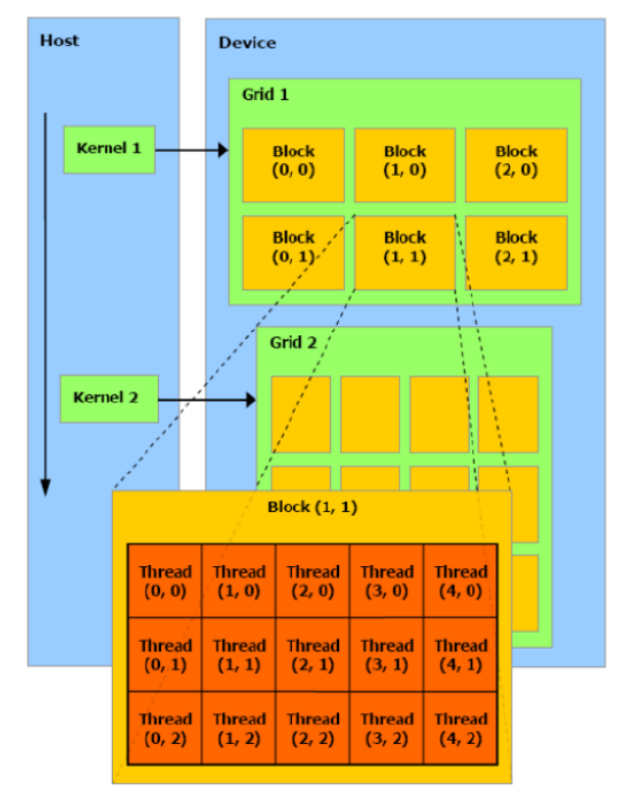
\includegraphics[width=0.6\textwidth]{pics/threads-organization.png}
	\caption{Организация потоков}
	\label{fig:threads-org}
\end{figure}

\subsection{Устройство памяти}

Графический процессор оснащён собственной глобальной памятью, которая не совпадает с оперативной памятью центрального процессора.

При выполнении кода на видеокарте обращение возможно лишь к её собственной памяти. Следовательно, для проведения вычислений и получения 
итогового результата требуется скопировать данные из оперативной памяти CPU в память GPU, а затем — обратно. Кроме того, каждый 
мультипроцессор помимо глобальной памяти располагает собственными кэшами, а также текстурной, константной, разделяемой памятью и так далее. 
Структура организации памяти в программах CUDA показана на рисунке \ref{fig:memory-org}.

\begin{figure}[H]
	\centering
	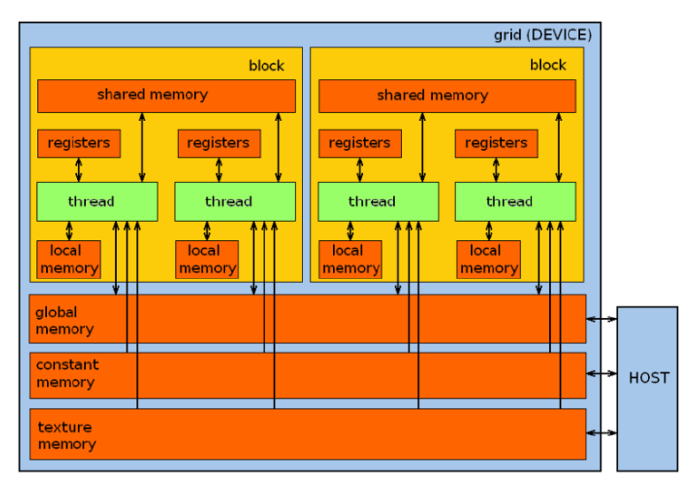
\includegraphics[width=0.6\textwidth]{pics/memory-org.png}
	\caption{Схема организации памяти CUDA-программы}
	\label{fig:memory-org}
\end{figure}

\subsection{Модели памяти}

В архитектуре CUDA различают шесть типов памяти:

\begin{enumerate}
\item \textbf{Регистры}

Компилятор по возможности старается размещать все локальные переменные функций именно в регистровой памяти. На каждый мультипроцессор 
приходится 8192 32-разрядных регистров, которые распределяются между нитями, выполняющимися на этом мультипроцессоре. Доступ к 
регистрам является самым быстрым.

\item \textbf{Локальная память}

Это небольшой объем памяти, доступный только одному потоковому процессору. В неё попадают локальные данные, имеющие слишком большой размер. 
Физически локальная память устроена так же, как глобальная, и работает с той же скоростью.

\item \textbf{Глобальная память}

Глобальная память обладает большим объёмом (от 256 Мбайт до 4 Гбайт). Она доступна для произвольного чтения и записи всем мультипроцессорам, 
а также центральному процессору (хосту). Однако эта память очень медленная и не кэшируется, поэтому количество обращений к ней следует 
минимизировать. Глобальная память физически расположена на хосте, тогда как разделяемая память — непосредственно на видеокарте. 
Из-за этого накладные расходы на передачу данных по шине для глобальной памяти выше, чем для разделяемой, хотя сами типы памяти по своей 
природе идентичны.

\item \textbf{Разделяемая память}

Разделяемая память не кэшируется, но работает быстро. Её рекомендуется использовать в качестве управляемого кэша. На один мультипроцессор 
выделяется всего 16 КБ разделяемой памяти. Она служит для взаимодействия между потоками, управляется непосредственно разработчиком и обладает 
малой задержкой. Отличительная особенность: разделяемая память адресуется одинаково для всех задач внутри блока, то есть её можно применять 
для обмена данными только между потоками одного блока.

\item \textbf{Константная память}

Константная память хранит неизменяемые данные, доступные на уровне всей сетки (grid). Её объём составляет 64 КБ, и физически она не отделена 
от глобальной памяти. Однако благодаря использованию кэшей и механизма широковещательной рассылки (broadcast) этот тип памяти может повысить 
производительность за счёт снижения трафика между процессором и памятью. Из-за небольшого объёма в ней имеет смысл размещать лишь небольшое 
количество часто используемых данных.

\item \textbf{Текстурная память}

Текстурная память похожа на константную: через текстурный блок возможны только операции чтения. Физически она также не отделена от глобальной. 
Как и константная, позволяет ускорить работу благодаря системе кэшей. Её отличительная черта — оптимизация текстурного кэша для двумерной 
пространственной локальности.

При вычислениях на модели в виде матрицы, когда соседние элементы взаимодействуют друг с другом, часто возникает необходимость обращаться к 
элементам окрестности некоторого элемента матрицы. С точки зрения адресации, элементы окрестности не расположены в памяти рядом друг с другом. 
Текстурная память позволяет кэшировать данные, основываясь на их пространственной, а не адресной локальности, то есть на том, что данные 
расположены близко в двумерном пространстве.

\end{enumerate}

\subsection{Модель вычислений на GPU}

Программа, предназначенная для выполнения на GPU с поддержкой NVIDIA CUDA, называется ядром (kernel). Ядро запускается одновременно на сетке, 
состоящей из блоков, каждый из которых включает несколько нитей (потоков). Количество блоков и число нитей в блоке задаются в момент вызова 
ядра. Все нити выполняют один и тот же код. Чтобы обеспечить разное поведение отдельных нитей, используется информация о номере блока и нити, 
которая доступна каждой нити.

С точки зрения графического процессора, понятия «поток» не существует — все команды, поступающие на GPU, обрабатываются в единой очереди для 
всех потоков.

Планировщик способен сглаживать порядок выполнения команд, одновременно запуская копирование данных с хоста, выполнение ядра и обратное 
копирование на хост. Если ядро загружает менее 50\% вычислительных ресурсов GPU, планировщик может запустить следующее ядро из другого потока, 
если оно готово к исполнению.

Для оптимизации времени выполнения задач в разных потоках важно учитывать, что команды на GPU выполняются в том порядке, в котором они были 
вызваны на хосте. Это означает, что не всегда эффективно полностью заполнять один поток задачами, затем второй и так далее. Более рациональный 
подход — равномерно распределять задачи по всем потокам.

Например, можно сначала отправить все команды в первый поток, а затем во второй. В таком случае команды второго потока будут ждать завершения 
команд первого. Альтернативный вариант — чередовать команды: отправить первую команду в первый поток, первую — во второй, затем вторую — в 
первый, вторую — во второй и так далее. Такое равномерное распределение позволяет повысить производительность, поскольку планировщик может 
одновременно запускать операции копирования и выполнения ядер.

\subsection{Компиляция программы}

Программы для видеокарт NVIDIA CUDA создаются на основе других языков программирования, в частности, используется расширение языка C, 
известное как CUDA C.

Для компиляции таких программ применяется компилятор nvcc, который входит в комплект инструментов разработчика. Данный набор инструментов, 
а также библиотеку CUDA можно загрузить с официального сайта NVIDIA.

\subsection{Планировщик задач}

Поток (stream) в CUDA представляет собой логическую цепочку зависимых асинхронных операций, которые выполняются независимо от операций в 
других потоках. Благодаря потокам можно отправлять команды CUDA на графический процессор в том порядке, который определён внутри контекста 
каждого отдельного потока.

С точки зрения GPU, потоки не существуют как самостоятельные объекты — все команды, поступающие на устройство, выстраиваются в общую для всех 
потоков очередь. Знание этой особенности может помочь при оптимизации производительности.

Планировщик способен сглаживать порядок исполнения: он может одновременно запускать копирование данных с хоста на устройство, копирование с 
устройства на хост и выполнение ядра. При вызове ядра можно указать, в какой поток его поместить. По умолчанию все ядра направляются в поток 0, 
который является синхронным по отношению к хосту. Если ядро загружает менее 50\% вычислительных ресурсов GPU, планировщик может запустить 
следующее ядро из другого потока при условии его готовности к выполнению.

Планировщик задач в CUDA — это механизм, управляющий исполнением потоков на GPU. Он отвечает за распределение ресурсов (вычислительных ядер, 
памяти и т.д.) между потоками и блоками. На рисунке \ref{fig:task-scheduler} показан планировщик задач для архитектуры Kepler.

\begin{figure}[H]
	\centering
	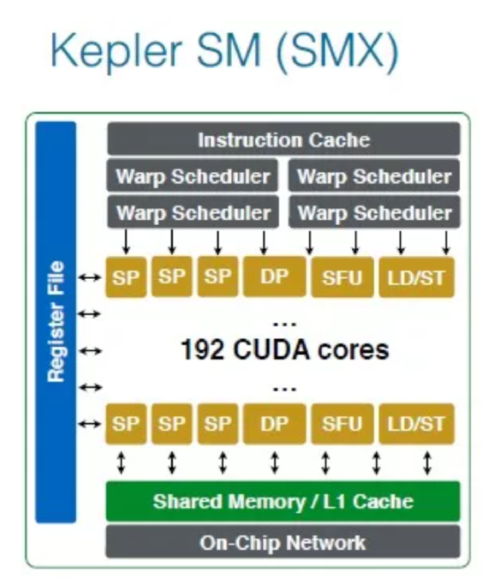
\includegraphics[width=0.3\textwidth]{pics/task-scheduler.png}
	\caption{Планировщик задач в архитектуре Kepler}
	\label{fig:task-scheduler}
\end{figure}

\pagebreak

\section{Суперкомпьютерный центр <<Политехнический>>}

\subsection{Состав}

В настоящий момент пользователям суперкомпьютерного центра «Политехнический» предоставлены следующие вычислительные мощности:

\begin{itemize}
\item 612 узлов кластера «Политехник – РСК Торнадо»;
\item 56 узлов кластера «Политехник – РСК Торнадо», оснащённых ускорителями NVIDIA K-40;
\item 288 узлов вычислительной системы с высокой степенью многопоточности «Политехник – РСК ПетаСтрим».
\end{itemize}

\subsection{Характеристики}

\begin{itemize}
\item Один узел кластера «Политехник – РСК Торнадо» оснащён:
  \begin{itemize}
    \item двумя процессорами Intel Xeon E5-2697 v3 с тактовой частотой 2.60 ГГц;
    \item 64 ГБ оперативной памяти.
  \end{itemize}

\item Один узел кластера «Политехник – РСК Торнадо» с графическими ускорителями NVIDIA K-40 включает:
  \begin{itemize}
    \item два процессора Intel Xeon E5-2697 v3 @ 2.60 ГГц;
    \item 64 ГБ RAM;
    \item два ускорителя Nvidia Tesla K40x с 12 ГБ видеопамяти GDDR.
  \end{itemize}

\item Один узел вычислителя «Политехник – РСК ПетаСтрим» содержит:
  \begin{itemize}
    \item один процессор Intel Xeon Phi 5120D с частотой 1.10 ГГц;
    \item 8 ГБ оперативной памяти.
  \end{itemize}
\end{itemize}

В качестве коммуникационной сети на всех доступных узлах используется InfiniBand со скоростью 56 Гбит/с (FDR). Кроме того, на всех узлах 
доступна параллельная файловая система Lustre объёмом около 1 петабайта.

По умолчанию пользователю предоставляется доступ к узлам \texttt{tornado}. Доступ к узлам других типов выдаётся по отдельному запросу.

\subsection{Технология подключения}

Для получения доступа зарегистрированному пользователю к суперкомпьютерному центру (СКЦ) следует применить любой терминальный клиент, 
поддерживающий протокол SSH. Это обеспечивает подключение к удалённому терминалу для работы с ресурсами СКЦ.

В рамках работы использовалась следующая процедура подключения:

\begin{enumerate}
	\item От администрации СКЦ были получены публичный и приватные ключи в виде файлов, а также логин пользователя для доступа к системе.
	\item Подготовка к подключению:
	
	\begin{itemize}
		\item Для организации подключения к СКЦ использовалась программа \texttt{OpenSSH}. На устройства с операционной системой MacOS Tahoe
		она предустановлена.
		\item Для обмена файлами использовался встроенный в операционную систему инструмент SFTP.
	\end{itemize}

	\item Для подключения к СКЦ необходимо ввести команду:
	
	\begin{lstlisting}
ssh -i .ssh/private-key login@login1.hpc.spbstu.ru
	\end{lstlisting}

	где:

	\begin{itemize}
		\item \texttt{login} --- логин для подключения к СКЦ;
		\item \texttt{login1.hpc.spbstu.ru} --- адрес узла СКЦ;
		\item \texttt{-i .ssh/private-key} --- по до приватного файла-ключа.
	\end{itemize}

	\item Для передачи файлов между используемой машиной и СКЦ требуются следующие параметры:
	
	Для входа:
	\begin{itemize}
		\item Имя хоста: \texttt{login1.hpc.spbstu.ru}
		\item Порт: 22
		\item Логин: \texttt{login}.
	\end{itemize}

	Для обмена данными:
	\begin{itemize}
		\item Навигация по удаленной системе:
		\begin{itemize}
			\item \texttt{pwd} --- показать текущую удалённую директорию.
			\item \texttt{cd имя\_папки} --— перейти в папку на сервере.
			\item \texttt{ls} --— список файлов на сервере (обычный или с ключами \texttt{ls -la}).
		\end{itemize}

		\item Навигация по локальной системе:
		\begin{itemize}
			\item \texttt{lpwd} --— показать текущую локальную директорию.
			\item \texttt{lcd путь} --— сменить локальную директорию (куда файлы будут скачиваться/откуда загружаться).
			\item \texttt{lls} --— список файлов на вашем компьютере.
		\end{itemize}

		\item Передача файлов:
		\begin{itemize}
			\item \texttt{get файл} --— скачать файл с сервера в текущую локальную папку.
			\item \texttt{get -r папка} —-- скачать папку целиком (рекурсивно).
			\item \texttt{put локальный\_файл} --— загрузить файл с вашего компьютера на сервер.
			\item \texttt{put -r папка} —-- загрузить папку со всем содержимым.
		\end{itemize}
	\end{itemize}
\end{enumerate}

В результате настройки было осуществлено подключение к СКЦ по протоколу SSH. На рисунке \ref{fig:start-page} представлена стартовая страница
при подключении к СКЦ.

\begin{figure}[H]
	\centering
	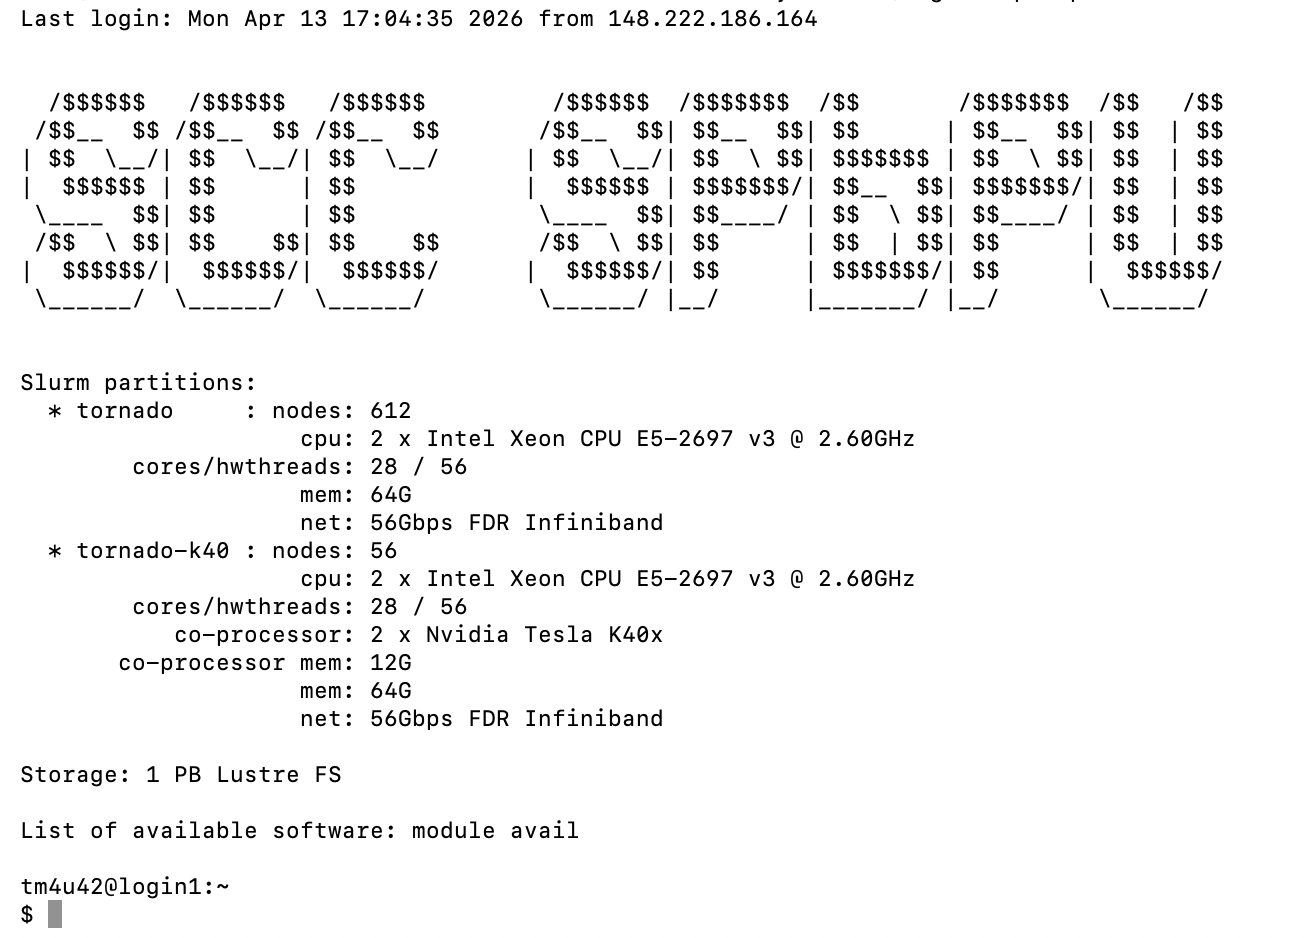
\includegraphics[width=0.8\textwidth]{pics/start-page.png}
	\caption{Стартовая страница при подключении к СКЦ}
	\label{fig:start-page}
\end{figure}

\pagebreak

\section{Постановка решаемой задачи}

Дано: 
\begin{itemize}
	\item массив $P$ --- полигон ($n \times n$) целых чисел. 
	\item $A$, $B$, $C$ --- координаты вершин треугольника в локальной системе координат. 
	\item $R$ --- радиус окружности. 
\end{itemize}

Требуется: вычислить $K_1$ --- число треугольников в массиве $P$, $K_2$ --- число окружностей в массиве $P$. 

\bigskip

Ограничения: 
\begin{itemize}
    \item границы контура треугольника в массиве $P$ --- $2$;
    \item границы контура окружности в массиве $P$ --- $3$;
    \item распределение треугольников и окружностей в массиве $P$ выполнено по случайному закону;
    \item $R=100$, треугольник $ABC$ равносторонний, длина стороны $>100$;
    \item треугольники и окружности в массиве $P$ могут пересекаться;
    \item значения элементов массива $P$ отличны от $2$ и $3$.
\end{itemize}
 
\pagebreak

\section{Алгоритм решения задачи}

Для вычисления $K_1$ и $K_2$ в условиях возможного пересечения контуров наиболее устойчивым методом является \textbf{Обобщенное преобразование Хафа}.

\subsubsection*{Предобработка данных}
Создадим две бинарные маски из исходного массива $P$:
\begin{itemize}
    \item $M_T(i, j) = 1$, если $P[i,j] = 2$ (контур треугольника);
    \item $M_C(i, j) = 1$, если $P[i,j] = 3$ (контур окружности).
\end{itemize}

\subsubsection*{Формирование эталонов (ядер)}
Определим множества относительных координат точек идеальных контуров:
\begin{enumerate}
    \item $\Delta_C$: координаты $(dx, dy)$ точек окружности $x^2 + y^2 = 100^2$.
    \item $\Delta_T$: координаты $(dx, dy)$ сторон равностороннего треугольника относительно его центра масс.
\end{enumerate}

\subsubsection*{Процедура голосования}
Для каждого типа фигуры выполняется следующий цикл накопления:

\begin{algorithmic}[1]
\State $Acc[n][n] \gets 0$ \Comment{Матрица аккумулятора}
\For{$x$ от 1 до $n$}
    \For{$y$ от 1 до $n$}
        \If{$M[x, y] == 1$}
            \For{каждого $(dx, dy) \in \Delta$}
                \State $cx = x - dx, cy = y - dy$
                \If{$(cx, cy)$ в границах массива}
                    \State $Acc[cx, cy] \gets Acc[cx, cy] + 1$
                \EndIf
            \EndFor
        \EndIf
    \EndFor
\EndFor
\State $K \gets \text{количество локальных максимумов в } Acc > \text{Порог}$
\end{algorithmic}

\subsubsection*{Обоснование параметров}
Так как фигуры могут пересекаться, часть пикселей одного контура может быть заменена пикселями другого. Установка порога обнаружения на 
уровне $80-90\%$ от общего числа точек эталона позволяет компенсировать эти потери и верно вычислить $K_1$ и $K_2$.


\subsection{Глобальная память}

\begin{enumerate}
    \item \textbf{Распределение потоков}
    \begin{itemize}
        \item Общее число элементов матрицы аккумулятора равно $N = n \times n$. Запускается одномерная 1D-сетка потоков.
        \item Индекс потока вычисляется как:
        \[ threadId = blockIdx.x \cdot blockDim.x + threadIdx.x \]
        \item Каждый поток обрабатывает элементы с индексами $idx = threadId + i \cdot T$, где $T$ — общее число потоков в сетке, при условии $idx < N$.
        \item Для каждого найденного контурного пикселя поток выполняет атомарную запись результатов в глобальную память.
    \end{itemize}

    \item \textbf{Алгоритм голосования}
    \begin{itemize}
        \item Координаты текущего пикселя вычисляются через линейный индекс:
        \[ row = \frac{idx}{n}, \quad col = idx \pmod n \]
        \item Если $P[row][col]$ соответствует контуру, выполняется цикл по шаблону $\Delta$:
        \[ Acc[row - dx][col - dy] = \sum atomicAdd(\dots) \]
    \end{itemize}
\end{enumerate}

\subsection{Разделяемая память}

\begin{enumerate}
    \item \textbf{Использование Shared Memory}
    \begin{itemize}
        \item Блок потоков копирует массив смещений шаблона $\Delta$ из глобальной памяти в разделяемую память блока для ускорения доступа:
        \[ shared\_delta[k] = delta[k] \]
        \item Синхронизация потоков внутри блока осуществляется через барьер \texttt{\_\_syncthreads()}.
    \end{itemize}

    \item \textbf{Сбор данных}
    \begin{itemize}
        \item Каждый поток вычисляется один элемент результирующей матрицы аккумулятора:
        \[ Acc[row][col] = \sum_{k=0}^{N_{\Delta}-1} M[row + shared\_delta[k].x][col + shared\_delta[k].y] \]
        где $M$ — бинарная маска соответствующей фигуры.
        \item Данный подход исключает использование атомарных операций, так как каждый поток пишет строго в свою ячейку памяти.
    \end{itemize}
\end{enumerate}

\pagebreak

\section{Описание эксперимента}

Цель эксперимента — оценка зависимости времени решения задачи от объема 
обрабатываемых данных и параметров запуска, связанных с GPU.

Для исследования времени решения задачи в зависимости от параметров были выбраны следующие параметры:

\begin{itemize}
    \item Используемая память: глобальная и разделяемая.
    \item Количество блоков: 1, 10, 100, 1000, 10000.
    \item Количество потоков в блоке: 32, 64, 128, 256, 512, 1024.
    \item Размеры полигона $P$: $1000 \times 1000$, $5000 \times 5000$, $10000 \times 10000$.
    \item Количество элементов в матрице: $10^4$, $10^6$, $2.5 \cdot 10^7$.
    \item Параметры фигур: радиус окружности $R=100$, сторона треугольника $>100$.
\end{itemize}

Для каждой комбинации параметров было проведено 100 измерений с помощью событий CUDA и взято среднее значение. 
Временные затраты на копирование данных между Host и Device в итоговых графиках учитывались отдельно от времени выполнения 
вычислительных ядер.

\pagebreak

\section{Анализ результатов}

На рисунке \ref{fig:results} представлены результаты эксперимента.

\begin{figure}[H]
	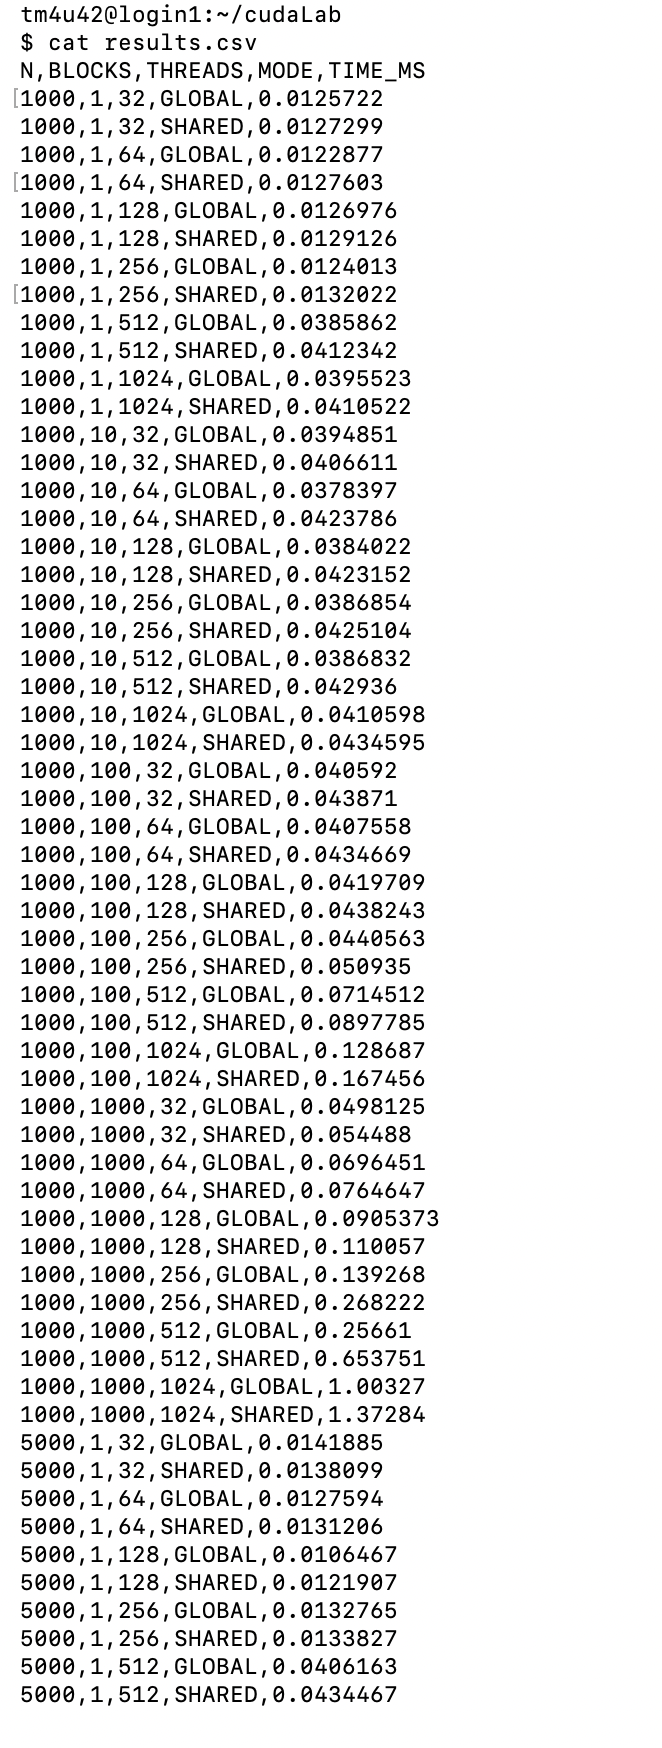
\includegraphics[width=0.48\textwidth]{pics/result1.png}
	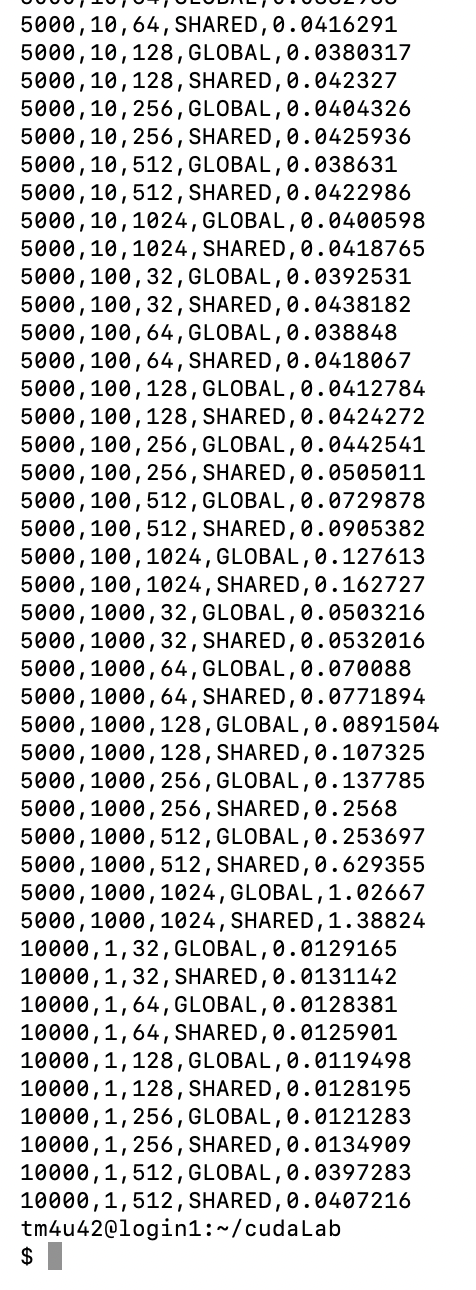
\includegraphics[width=0.48\textwidth]{pics/result2.png}
	\caption{Результаты эксперимента}
	\label{fig:results}
\end{figure}

В таблицах 1-3 представлены усредненные результаты работы алгоритма с использованием глобальной памяти.

\begin{table}[H]
\centering
\caption{Усредненные результаты измерения времени исполнения программы для матрицы $1000 \times 1000$ и глобальной памяти (мс)}
\label{tab:time-1000-global}
\begin{tabular}{lcccc}
\toprule
\textbf{Число потоков в блоке} & \multicolumn{4}{c}{\textbf{Число блоков}} \\
\cmidrule(lr){2-5}
 & 1 & 10 & 100 & 1000 \\
\midrule
32   & 0.0134 & 0.0407 & 0.0410 & 0.0501 \\
64   & 0.0112 & 0.0410 & 0.0395 & 0.0702 \\
128  & 0.0115 & 0.0388 & 0.0399 & 0.0894 \\
256  & 0.0128 & 0.0389 & 0.0429 & 0.1399 \\
512  & 0.0391 & 0.0400 & 0.0727 & 0.2538 \\
1024 & 0.0390 & 0.0391 & 0.1298 & 1.0008 \\
\bottomrule
\end{tabular}
\end{table}


\begin{figure}[H]
	\centering
	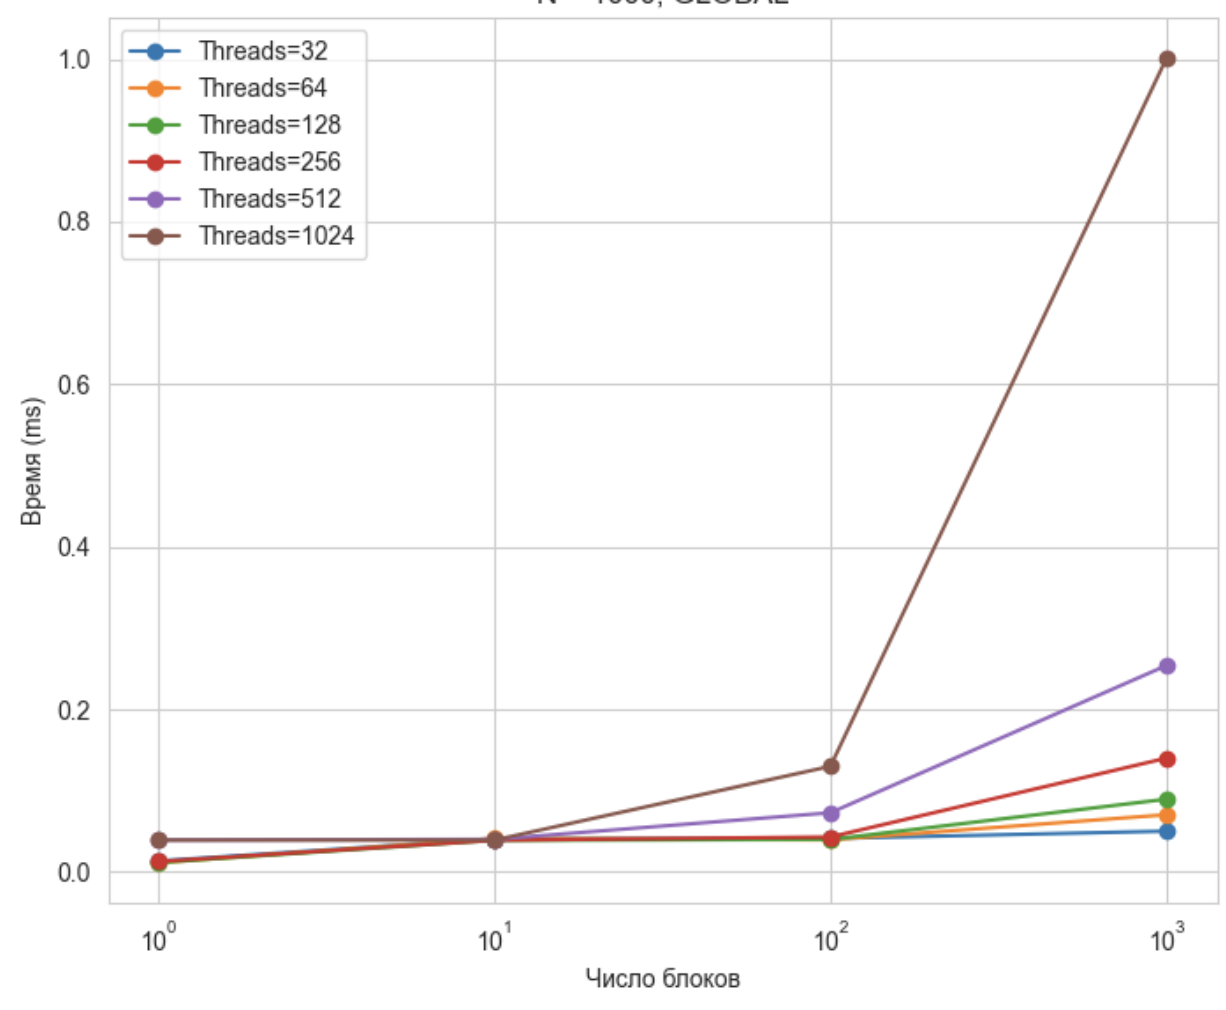
\includegraphics[width=0.8\textwidth]{pics/global1.png}
	\caption{График результатов времени исполнения программы для матрицы $1000 \times 1000$}
\end{figure}

\begin{table}[H]
\centering
\caption{Усредненные результаты измерения времени исполнения программы для матрицы $5000 \times 5000$ и глобальной памяти (мс)}
\label{tab:time-5000-global}
\begin{tabular}{lcccc}
\toprule
\textbf{Число потоков в блоке} & \multicolumn{4}{c}{\textbf{Число блоков}} \\
\cmidrule(lr){2-5}
 & 1 & 10 & 100 & 1000 \\
\midrule
32   & 0.0131 & 0.0399 & 0.0398 & 0.0485 \\
64   & 0.0130 & 0.0391 & 0.0400 & 0.0695 \\
128  & 0.0129 & 0.0388 & 0.0418 & 0.0886 \\
256  & 0.0112 & 0.0398 & 0.0446 & 0.1397 \\
512  & 0.0395 & 0.0396 & 0.0728 & 0.2525 \\
1024 & 0.0381 & 0.0402 & 0.1279 & 1.0233 \\
\bottomrule
\end{tabular}
\end{table}

\begin{figure}[H]
	\centering
	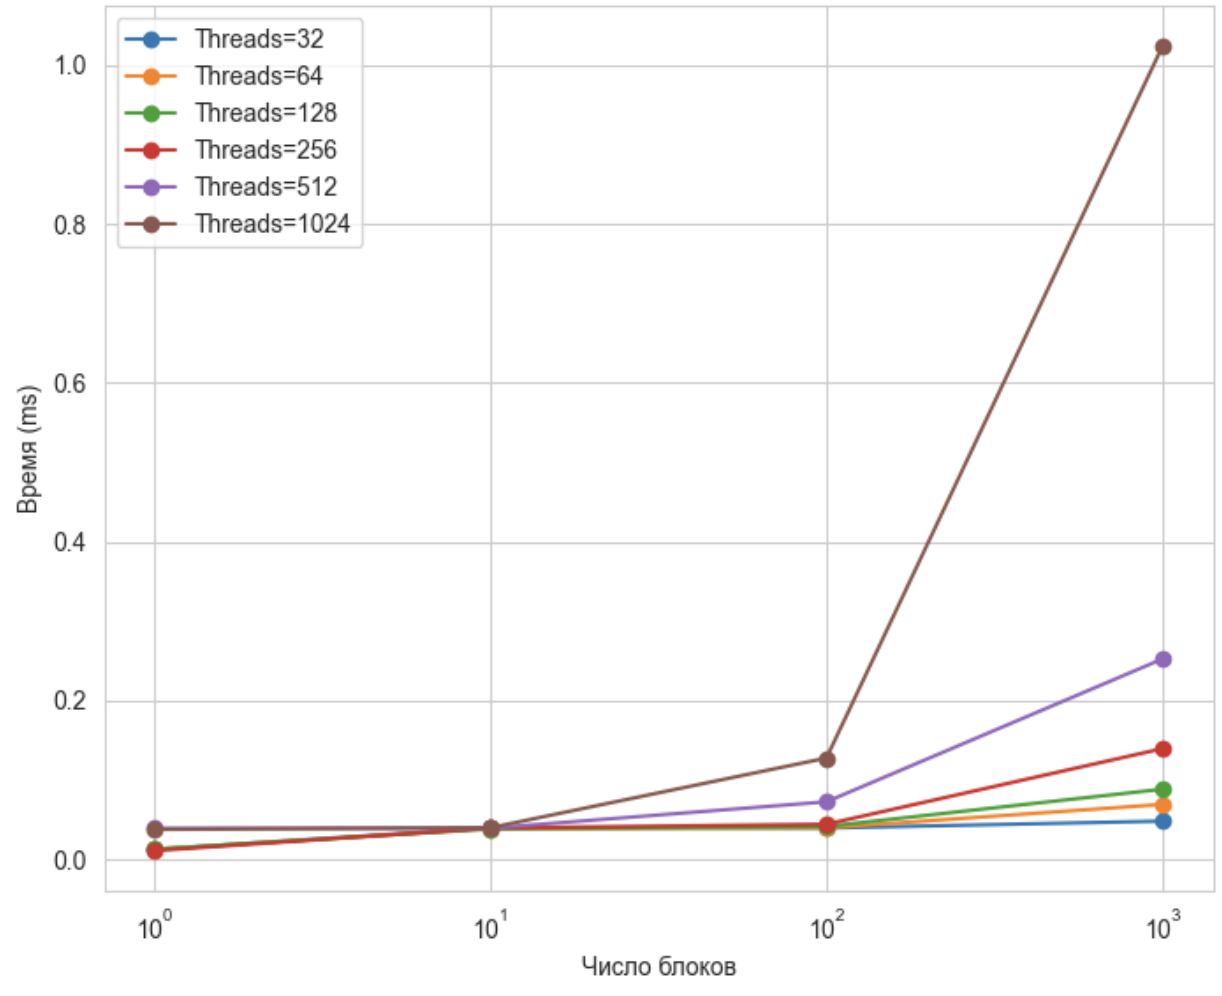
\includegraphics[width=0.8\textwidth]{pics/global2.png}
	\caption{График результатов времени исполнения программы для матрицы $5000 \times 5000$}
\end{figure}

\begin{table}[H]
\centering
\caption{Усредненные результаты измерения времени исполнения программы для матрицы $10000 \times 10000$ и глобальной памяти (мс)}
\label{tab:time-10000-global}
\begin{tabular}{lcccc}
\toprule
\textbf{Число потоков в блоке} & \multicolumn{4}{c}{\textbf{Число блоков}} \\
\cmidrule(lr){2-5}
 & 1 & 10 & 100 & 1000 \\
\midrule
32   & 0.0132 & 0.0389 & 0.0415 & 0.0488 \\
64   & 0.0109 & 0.0392 & 0.0393 & 0.0695 \\
128  & 0.0110 & 0.0388 & 0.0408 & 0.0894 \\
256  & 0.0130 & 0.0398 & 0.0442 & 0.1379 \\
512  & 0.0396 & 0.0406 & 0.0726 & 0.2520 \\
1024 & 0.0387 & 0.0399 & 0.1276 & 1.0155 \\
\bottomrule
\end{tabular}
\end{table}

\begin{figure}[H]
	\centering
	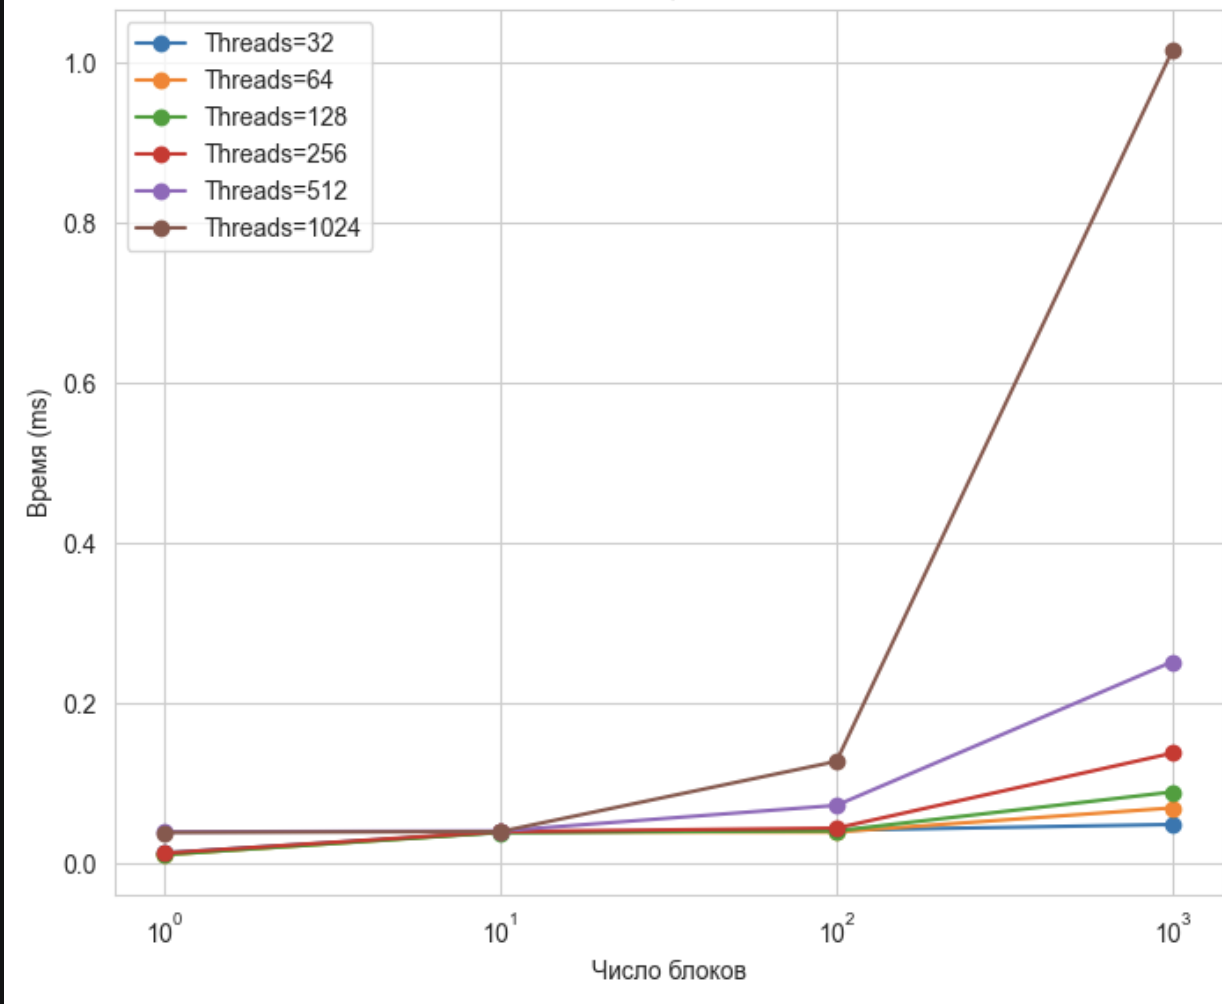
\includegraphics[width=0.8\textwidth]{pics/global3.png}
	\caption{График результатов времени исполнения программы для матрицы $10000 \times 10000$}
\end{figure}

В таблицах 4-6 представлены усредненные результаты работы алгоритма с использованием глобальной и разделяемой памяти.

\begin{table}[H]
\centering
\caption{Усредненные результаты измерения времени исполнения программы для матрицы $1000 \times 1000$ и разделяемой памяти (мс)}
\label{tab:time-1000-shared}
\begin{tabular}{lcccc}
\toprule
\textbf{Число потоков в блоке} & \multicolumn{4}{c}{\textbf{Число блоков}} \\
\cmidrule(lr){2-5}
 & 1 & 10 & 100 & 1000 \\
\midrule
32   & 0.0135 & 0.0430 & 0.0422 & 0.0532 \\
64   & 0.0131 & 0.0425 & 0.0407 & 0.0786 \\
128  & 0.0115 & 0.0409 & 0.0447 & 0.1087 \\
256  & 0.0130 & 0.0437 & 0.0524 & 0.2678 \\
512  & 0.0420 & 0.0444 & 0.0912 & 0.6505 \\
1024 & 0.0414 & 0.0432 & 0.1691 & 1.3692 \\
\bottomrule
\end{tabular}
\end{table}

\begin{figure}[H]
	\centering
	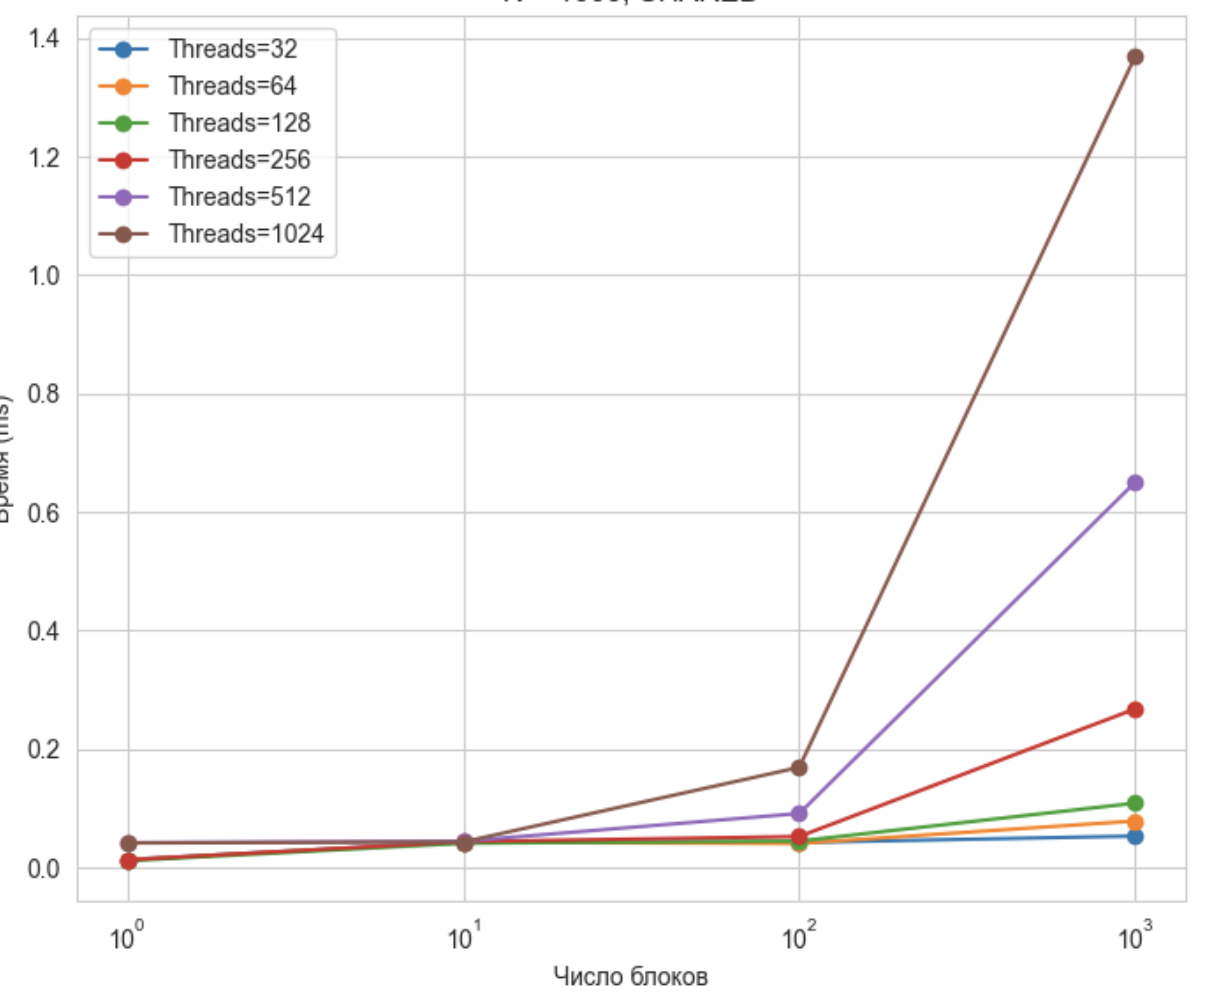
\includegraphics[width=0.8\textwidth]{pics/shared1.png}
	\caption{График результатов времени исполнения программы для матрицы $1000 \times 1000$}
\end{figure}

\begin{table}[h!]
\centering
\caption{Усредненные результаты измерения времени исполнения программы для матрицы $5000 \times 5000$ и разделяемой памяти (мс)}
\label{tab:time-5000-shared}
\begin{tabular}{lcccc}
\toprule
\textbf{Число потоков в блоке} & \multicolumn{4}{c}{\textbf{Число блоков}} \\
\cmidrule(lr){2-5}
 & 1 & 10 & 100 & 1000 \\
\midrule
32   & 0.0120 & 0.0437 & 0.0415 & 0.0514 \\
64   & 0.0133 & 0.0408 & 0.0423 & 0.0758 \\
128  & 0.0133 & 0.0424 & 0.0447 & 0.1062 \\
256  & 0.0111 & 0.0420 & 0.0528 & 0.2579 \\
512  & 0.0429 & 0.0416 & 0.0904 & 0.6266 \\
1024 & 0.0431 & 0.0430 & 0.1627 & 1.3838 \\
\bottomrule
\end{tabular}
\end{table}

\begin{figure}[H]
	\centering
	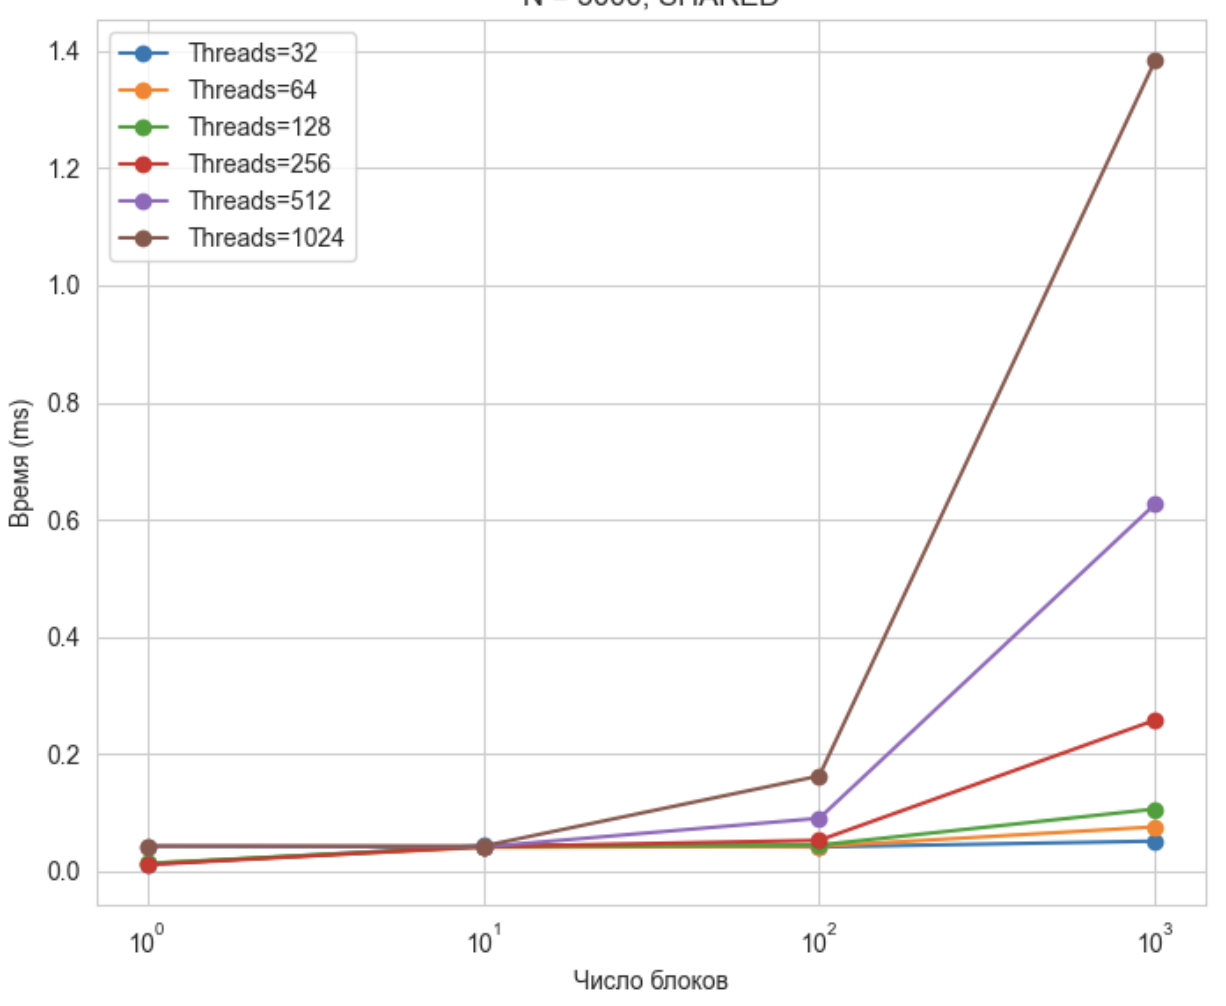
\includegraphics[width=0.8\textwidth]{pics/shared2.png}
	\caption{График результатов времени исполнения программы для матрицы $5000 \times 5000$}
\end{figure}

\begin{table}[h!]
\centering
\caption{Усредненные результаты измерения времени исполнения программы для матрицы $5000 \times 5000$ и разделяемой памяти (мс)}
\label{tab:time-10000-shared}
\begin{tabular}{lcccc}
\toprule
\textbf{Число потоков в блоке} & \multicolumn{4}{c}{\textbf{Число блоков}} \\
\cmidrule(lr){2-5}
 & 1 & 10 & 100 & 1000 \\
\midrule
32   & 0.0124 & 0.0410 & 0.0427 & 0.0546 \\
64   & 0.0132 & 0.0413 & 0.0419 & 0.0758 \\
128  & 0.0118 & 0.0418 & 0.0436 & 0.1061 \\
256  & 0.0120 & 0.0407 & 0.0534 & 0.2546 \\
512  & 0.0434 & 0.0430 & 0.0900 & 0.6158 \\
1024 & 0.0432 & 0.0425 & 0.1624 & 1.3465 \\
\bottomrule
\end{tabular}
\end{table}

\begin{figure}[H]
	\centering
	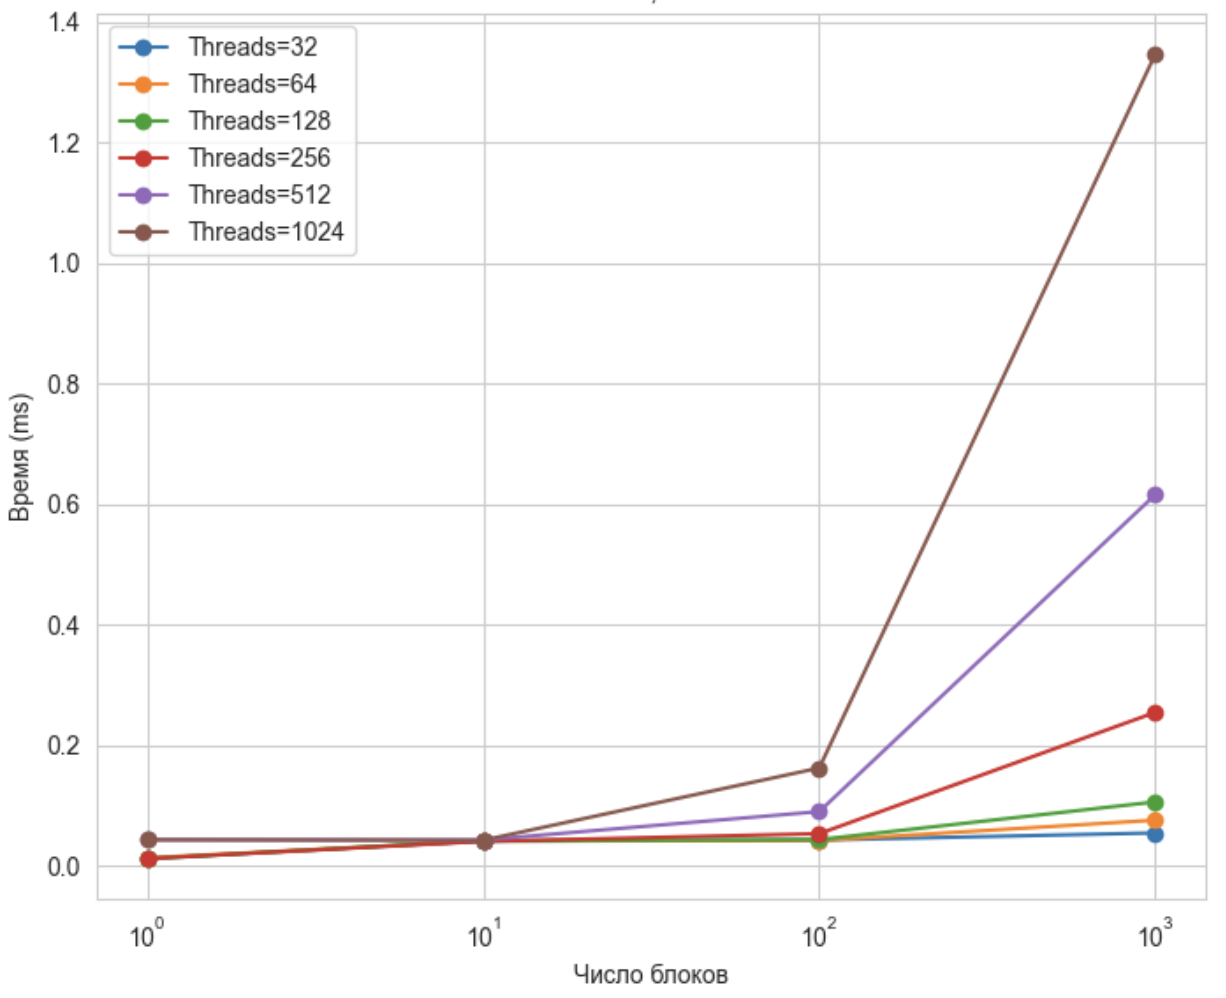
\includegraphics[width=0.8\textwidth]{pics/shared3.png}
	\caption{График результатов времени исполнения программы для матрицы $5000 \times 5000$}
\end{figure}

\subsection*{Зависимость от размера полигона}

Для анализа влияния размера полигона на время выполнения сопоставим результаты, полученные для $N = 1000, 5000, 10\,000$ (таблицы~\ref{tab:time-1000-global}--\ref{tab:time-10000-shared}).  
В отличие от интуитивных ожиданий, в исследованном диапазоне время исполнения практически не зависит от линейного размера полигона.

\begin{itemize}
    \item \textbf{Минимальное время (глобальная память).}  
    Для $N = 1000$ наименьшее время составило $0.0112$~мс (64 потока, 1 блок);  
    для $N = 5000$ --- также $0.0112$~мс (256 потоков, 1 блок);  
    для $N = 10\,000$ --- $0.0109$~мс (64 потока, 1 блок).  
    Разброс составляет менее $3\%$ и лежит в пределах погрешности измерений.

    \item \textbf{Минимальное время (разделяемая память).}  
    Аналогичная картина наблюдается и для режима совместного использования глобальной и разделяемой памяти:  
    $0.0115$~мс ($N=1000$), $0.0111$~мс ($N=5000$), $0.0118$~мс ($N=10\,000$).

    \item \textbf{Максимальное время (наихудшая конфигурация).}  
    Даже при максимальной загрузке GPU (1000 блоков, 1024 потока) время остаётся практически постоянным:  
    глобальная память --- $1.0008$~мс, $1.0233$~мс, $1.0155$~мс;  
    разделяемая память --- $1.3692$~мс, $1.3838$~мс, $1.3465$~мс.  
    Ни в одном случае не наблюдается пропорционального роста времени с увеличением $N$.
\end{itemize}

\subsection*{Зависимость от числа блоков и потоков}

Результаты, представленные в таблицах~\ref{tab:time-1000-global}--\ref{tab:time-10000-shared}, показывают, что время выполнения в исследованной задаче определяется главным образом конфигурацией запуска ядра, а не объёмом вычислений.  
В отличие от интенсивных вычислительных задач, где увеличение числа потоков приводит к пропорциональному сокращению времени, в нашем случае накладные расходы на планирование и синхронизацию доминируют.

\begin{itemize}
    \item \textbf{Влияние числа потоков в блоке.}  
    При малом количестве блоков (1--10) время практически не зависит от числа потоков, оставаясь в диапазоне $0.011\ldots0.043$~мс для любой конфигурации.  
    С ростом числа блоков чувствительность к числу потоков резко возрастает.  
    Например, для глобальной памяти при $N=1000$ и 1000 блоках время увеличивается с $0.0501$~мс (32 потока) до $1.0008$~мс (1024 потока), т.е. почти в 20 раз.  
    Это объясняется тем, что большое число потоков в сочетании с большим числом блоков создаёт чрезмерную нагрузку на планировщик GPU и ограниченные аппаратные ресурсы (регистры, разделяемая память), что приводит к сериализации исполнения.

    \item \textbf{Влияние числа блоков.}  
    При фиксированном числе потоков увеличение блоков до 100 почти не меняет время; заметный рост начинается только при 1000 блоках.  
    Особенно сильно этот эффект выражен для конфигураций с 512 и 1024 потоками.  
    Так, при 1024 потоках время выполнения для глобальной памяти и $N=1000$ составляет $0.0390$~мс (1 блок), $0.1298$~мс (100 блоков) и $1.0008$~мс (1000 блоков).  
    Следовательно, количество блоков начинает играть негативную роль, когда суммарное число потоков превышает возможности эффективного планирования на конкретном GPU.

    \item \textbf{Оптимальная конфигурация.}  
    Минимальное время во всех экспериментах достигается при использовании единственного блока и числа потоков 64 или 128.  
    Эта комбинация избегает заметных накладных расходов на запуск блоков и синхронизацию, обеспечивая задержку на уровне $0.011$~мс.  
    Дальнейшее увеличение числа блоков или потоков не приводит к сокращению времени, а лишь добавляет паразитные затраты.
\end{itemize}


\subsection*{Сравнение глобальной и разделяемой памяти}

Результаты сравнения двух подходов к организации памяти для всех исследованных размеров полигона сведены в таблице~\ref{tab:minmax}.

\begin{table}[H]
\centering
\caption{Максимальное и минимальное время для каждого размера и типа памяти}
\label{tab:minmax}
\begin{tabular}{cclcrc}
\toprule
\textbf{Размер $N$} & \textbf{Тип памяти} & \textbf{Мин/макс} & \textbf{Время (мс)} & \textbf{Блоки} & \textbf{Потоки} \\
\midrule
$1000$    & Глобальная  & Максимальное & $1.0008$ & $1000$ & $1024$ \\
          &             & Минимальное  & $0.0112$ & $1$    & $64$   \\
          & Разделяемая & Максимальное & $1.3692$ & $1000$ & $1024$ \\
          &             & Минимальное  & $0.0115$ & $1$    & $128$  \\
\midrule
$5000$    & Глобальная  & Максимальное & $1.0233$ & $1000$ & $1024$ \\
          &             & Минимальное  & $0.0112$ & $1$    & $256$  \\
          & Разделяемая & Максимальное & $1.3838$ & $1000$ & $1024$ \\
          &             & Минимальное  & $0.0111$ & $1$    & $256$  \\
\midrule
$10000$   & Глобальная  & Максимальное & $1.0155$ & $1000$ & $1024$ \\
          &             & Минимальное  & $0.0109$ & $1$    & $64$   \\
          & Разделяемая & Максимальное & $1.3465$ & $1000$ & $1024$ \\
          &             & Минимальное  & $0.0118$ & $1$    & $128$  \\
\bottomrule
\end{tabular}
\end{table}

Анализ таблицы~\ref{tab:minmax} и детальных таблиц~\ref{tab:time-1000-global}--\ref{tab:time-10000-shared} показывает, что в исследованной задаче использование разделяемой памяти не даёт выигрыша в производительности ни при одном из рассмотренных размеров полигона.  
Напротив, во всех случаях минимальное время для разделяемой памяти либо практически совпадает с глобальным, либо немного хуже, а максимальное время всегда больше для разделяемой памяти.

\begin{itemize}
    \item \textbf{Малые накладные расходы при 1 блоке.}  
    Для единственного блока разница во времени между глобальной и разделяемой памятью пренебрежимо мала.  
    Это объясняется тем, что при таком запуске синхронизация и загрузка данных в разделяемую память выполняются лишь одним блоком, а сама работа настолько мала, что задержки памяти не являются узким местом.

    \item \textbf{Рост накладных расходов с увеличением параллелизма.}  
    С ростом числа блоков и потоков накладные расходы разделяемой памяти резко возрастают.  
    Например, при $1000$ блоках и $1024$ потоках для $N=1000$ время для разделяемой памяти ($1.3692$~мс) на $\sim37\%$ выше, чем для глобальной ($1.0008$~мс), а для $N=5000$ это превышение достигает $35\%$.  
    Причина в том, что дополнительные операции синхронизации и копирования данных из глобальной памяти в разделяемую становятся доминирующим фактором при большом количестве одновременно работающих блоков.

    \item \textbf{Отсутствие выгоды от ускоренного доступа.}  
    Хотя время доступа к разделяемой памяти на порядок меньше, чем к глобальной, в данной задаче каждый поток использует данные лишь однократно (или малое число раз), поэтому преимущества разделяемой памяти не успевают проявиться.  
    Положительный эффект от быстрого доступа полностью нивелируется временем, затраченным на её инициализацию и барьерную синхронизацию.

    \item \textbf{Зависимость от размера полигона не выявлена.}  
    Даже для самого большого размера $N=10000$ разделяемая память не даёт преимущества, что отличает данную задачу от многих классических GPU-алгоритмов (например, умножения матриц или свёрток), где с ростом объёма данных выигрыш от разделяемой памяти становится заметнее.
\end{itemize}

Таким образом, в рамках проведённого эксперимента оптимальной стратегией является использование глобальной памяти с минимальным числом блоков и умеренным числом потоков.  
Разделяемая память лишь добавляет накладные расходы, не обеспечивая выигрыша в скорости, и её применение в аналогичных лёгких ядрах следует считать нецелесообразным.

\pagebreak

\section*{Заключение}
\addcontentsline{toc}{section}{Заключение}

В ходе данной курсовой работы была изучена технология параллельного программирования на основе архитектуры NVIDIA CUDA.  
В теоретической части был проведён обзор архитектуры CUDA, включая её вычислительные возможности, иерархию памяти и модель исполнения на графических процессорах NVIDIA.  

\medskip

В практической части работы:
\begin{itemize}
    \item Реализовано и распараллелено ядро на языке CUDA C для вычисления числа треугольников и окружностей на полигоне.
    \item Проведена отладка на локальной машине с поддержкой CUDA.
    \item Финальная серия экспериментов выполнена на суперкомпьютере «Политехнический» с использованием вычислительного узла «Политехник‑РСК Торнадо» (графический ускоритель NVIDIA K40).
    \item Варьировались следующие параметры: размер полигона ($N = 1000, 5000, 10\,000$), число блоков (1, 10, 100, 1000), число потоков в блоке (32, 64, 128, 256, 512, 1024), тип используемой памяти (глобальная, глобальная + разделяемая).
\end{itemize}

Основные выводы по результатам эксперимента:

\begin{enumerate}
    \item \textbf{Время выполнения не зависит от размера полигона} в исследованном диапазоне $N$.  
    И глобальная, и разделяемая память показали практически одинаковые значения минимального и максимального времени для всех трёх размеров. Это свидетельствует о том, что вычислительная нагрузка на поток пренебрежимо мала, а доминируют накладные расходы на запуск и синхронизацию.

    \item \textbf{Использование разделяемой памяти не дало выигрыша в производительности}.  
    Для всех конфигураций время с разделяемой памятью было либо практически равно времени с глобальной памятью (при малом числе блоков), либо заметно выше (при 1000 блоках и большом числе потоков). Причина — в лёгком ядре время копирования данных в разделяемую память и барьерная синхронизация не окупаются более быстрым доступом.

    \item \textbf{Оптимальной стратегией является минимизация параллелизма}.  
    Минимальное время во всех случаях достигается при использовании одного блока и 64–256 потоков. Увеличение числа блоков до 1000 или потоков до 1024 приводит к многократному росту времени из‑за конкуренции за ресурсы GPU и издержек планирования.

    \item \textbf{Конфигурация с одним блоком и умеренным числом потоков является наилучшей} для исследованного класса задач. Широко распространённый подход, при котором произведение числа блоков на число потоков должно примерно равняться числу элементов, в данном случае неэффективен именно из‑за крайне низкой полезной нагрузки на один поток.
\end{enumerate}

Таким образом, для лёгких CUDA‑ядер с малым объёмом вычислений на поток ключевым фактором становится не пропускная способность памяти или пиковая производительность GPU, а минимизация накладных расходов. Результаты работы показывают, что в подобных ситуациях следует отдавать предпочтение глобальной памяти и небольшому числу потоковых блоков, избегая избыточного распараллеливания.

\pagebreak

\begin{thebibliography}{99}

\bibitem{sanders} Сандерс, Д. Технология CUDA в примерах: введение в программирование графических процессоров. — М: ДМК Пресс, 2013. — 232 с.

\bibitem{politech_guide} Краткое руководство пользователя вычислителей «Политехник - РСК Торнадо» и «Политехник - РСК Пегастрим».

\bibitem{scc_spbstu} Суперкомпьютерный центр — Ресурсы СКЦ. // Суперкомпьютерный центр «Политехнический». [Электронный ресурс]. – Режим доступа: URL: https://scc.spbstu.ru/resources (дата обращения: 20.03.2026).

\end{thebibliography}

\end{document}